\documentclass[a4paper, 12pt]{report}
\usepackage{fullpage}
\usepackage{graphicx}
\usepackage{float}
\usepackage{fixltx2e}
\usepackage{rotating}
\usepackage{textcomp}

\begin{document}
\begin{titlepage}
\begin{center}

\LARGE{Electronics and Computer Science}\\
\LARGE{Department of Physical and Applied Sciences}\\
\LARGE{University of Southampton}\\
\vfill
\normalsize{Thomas Scarsbrook}
\vfill
\normalsize\today

\vfill

\normalsize{Supervisor: Steve Gunn}\\
\normalsize{Examiner: Rob Maunder}

\vfill

\large{A project progress report submitted for the award of\\
MEng Electronic Engineering with Mobile and Secure Systems}

\end{center}
\end{titlepage}


\abstract{There are many undesired sounds around us all the time.
These sounds can often be very distracting to what we are attempting to hear.
There are various methods we can employ in an attempt to reduce the effect of these undesired sounds
So far I have experimented with one method of cancelling these out with a measured amount of success, however it is not optimal and suffers from some physical limitations.
I am also looking into an alternative, potentially much faster method of achieving the cancellation.
}
\addcontentsline{toc}{section}{Abstract}
\setcounter{page}{2}

\tableofcontents
\addcontentsline{toc}{section}{Contents}

\listoffigures
\addcontentsline{toc}{section}{List of Figures}

\listoftables
\addcontentsline{toc}{section}{List of Tables}

\chapter*{Acknowledgements}
I would like to thank my supervisor Steve Gunn for all his support and advice
during this project.
I would also like to thank the members of Student Robotics, who not only helped
me come up with the idea of this project, but also introduced me to many of the
pieces of software used in the project.
Also there are all the people who assisted with the proof reading of the
reports, including a couple of the people on my course, my parents, and some of
my sixth form teachers.

\addcontentsline{toc}{section}{Acknowledgements}

This is text \cite{EMHeadsets}
This is other text \cite{EMNoiseCancel}

This is more \cite{ICAAlg&Apps} text\\
Then you get some text about psychoacoustics \cite{MusCogCompSou} and about the DELAYS in sound waves, and how the ear uses them.

WOW, THIS SOURCE\cite{AdvancedDSPing} IS FANTSATIC, Shame that it seems innaccesable without spending \textsterling50\ldots \\
I especially reccommend looking at Page 12, it contains a great diagram!

\chapter{Introduction}
\newpage
\section{Project Description}
The aim of this project is to produce the electronics for a set of headphones which will be capable of detecting and cancelling an unwanted sound source from that being heard by the user.


\chapter{Background}

\section{Alternatives}

There are many varieties of noise cancelling headphones available on the market, and many different methods are employed in order to achieve the cancellation.
Noise cancelling headphones have been in production for years due to the demand to reduce the surrounding sounds, for example to protect paramedics hearing whilst in an ambulance \cite{EMHeadsets}, or to improve music quality.

\subsection{Methods}
Out of all the methods of achieving noise cancellation, the most primitive is to use Ear Canal Headphones (ECH).
These physically isolate the eardrum from the external noise sources.
The advantages of this method are that no electronic parts are required, as all the attenuation is achieved passively, however this dulls out all noise and can result in the user being apparently deaf.
\\
\\
The majority of methods use active noise cancelling (ANC), whereby some electronics are used to cancel out the noise.
These devices come in a variety of forms, and may be capable of just cancelling certain parts of the frequency spectrum rather than all sounds.
ANC technology produces a cancelling signal of the same amplitude to the noise, however with a phase shift of 180$^{\circ}$.
When superimposed on the sound reaching the ear, this anti-phase signal causes the noise to be cancelled away, as such the user does not hear it.
With ANC methods, passive cancelling is generally not employed, partially as it attenuates the sounds between the feed-forward sensor and the users ear, meaning that the cancellation signal is of a greater magnitude at the eardrum that the signal it is cancelling.
Over cancelling like this results in the noise to be reproduced, albeit 180$^{\circ}$ out of phase and heavily attenuated.
The most basic method for producing this cancellation signal is to produce a unity gain, inverting amplifier and add the signal to the headphone output.
One system that uses such an implementation is covered in section \ref{sec:philipsphones}.
\\
\\
Such methods are limited in their capabilities as additional phase shifts or attenuations can be caused by the construction of the headphones.
One option for accounting for this is to use a feedback sensor instead of feed-forward.
This prevents over cancellation and accounts for any multipath traits the noise might exhibit.
The issue with such a design is that they remove all sound, and it is not possible to then introduce an additional, desired sound, potentially from an MP3 player or similar.
Sounds from the desired source will be detected at the feedback microphone, along with the noise sounds, and a cancelling signal designed to cancel both the noise and the desired signals will be produced.
Therefore, this design is suitable for ear defenders for workers in a factory, however would not be suitable for a pilot requiring to hear the radio over the engine noise.
\\
\\
Another way to deal with this is to introduce a second microphone \cite{EMNoiseCancel,2SensorANCAlg} in order that both feed-forward and feedback can be provided.
To generate the cancelling signal, only the feed-forward signal gets used, with the feedback signal allowing the effectiveness of the cancelling to be measured as a power level.
This allows the cancelling to be achieved stably, without cancelling the desired signals.
\\
\\
\nocite{*}
In \cite{EMHeadsets} it is possible to see the use of a DSP in order to achieve cancelling, where only a specific range of noise signals are attenuated.
This method employs signal conditioning filters to remove frequencies outside the range of the noise signal.
This is made possible by prior knowledge of the type of noise signal.
It is known that the siren is between $400-800Hz$, and as such only sounds inside this frequency range require cancellation.
Because of this a low power DSP is possible, along with a lower sampling rate, allowing a longer battery life for the supporting circuitry.
One notable feature with the design in \cite{EMHeadsets} is that there is no feed-forward, the system is based purely around feedback.
As a result only the sound actually reaching the users ear is cancelled, rather than a prediction from a feed-forward mechanism.
Furthermore the system is more stable.
The methodology used here is to use the DSP to implement a LMS adaptive filter, taking the filtered feedback signal as an input.
\\
\\
One major issue with ANC is the stability of the control system.
It is very easy to create a situation whereby the algorithm is unstable, or the cancellation achieved is suboptimal.
Sources \cite{AuralEnvironmentAdjANC} and \cite{ANCOptimalControlInf} look at two methods in which to combat this.

\subsection{Differences to this Project}
All of these methodologies take in the noise source that is reaching the users ear and apply a cancellation signal to remove all of the sound.
Some of the more advanced methods use a second sound input, which is essentially feedback, allowing the cancellation to be increase in optimality.
None of these methods allow for only a single component to be cancelled, the cancelling signal is produced for all sound reaching the ear.
This project aims to address this, and provide this ability in order to achieve all the benefits of the alternative methods without removing sounds that are required.
Furthermore, this project aims to achieve this without feedback, in order to allow ear bud style headphones to be used to increase convenience to the user.
Extra processing is required for the detection of one signal inside the heard sounds, however allows for the methodology to be used in circumstances where feedback may not be possible.
Also, the lack of feedback allows for the demanded signal to be guaranteed.
The reasoning for this is covered in section \ref{text:virtualfeedbackassumption}.
One such circumstance could be where the cancellation is attempted remotely, without any contact with the user.
This could be something like reducing the noise sounds from speakers in a theater entrance, allowing the box office attendants and late arrivals to communicate with each other, while not having to wear headsets.
One of the methods used in this project is supported by \cite{EMHeadsets,EMNoiseCancel,2SensorANCAlg}, showing that the LMS approach is a tested and proven method for ANC.
The use of LMS will be discussed in section \ref{sec:planlms}.


\section{Consumer Headphones}
There are many consumer noise cancelling headphones, with various means of doing the cancellation. One of the cheaper versions available are Philips SHN2500.
These headphones use a rather significantly different approach to achieving the detection and cancelling than my method. Reverse engineering the circuit in these headphones reveals the schematic as shown in figure \ref{fig:philipsphonessche}.

\begin{figure}[h]
	\centering
	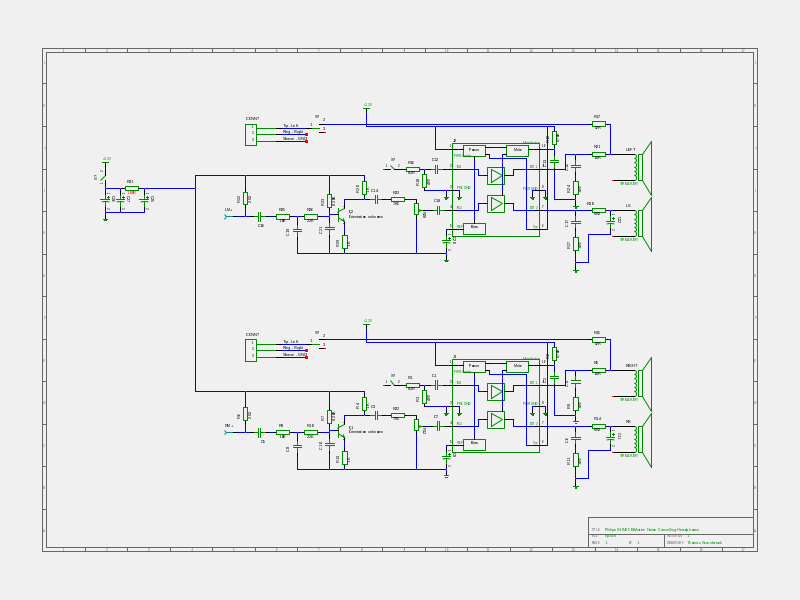
\includegraphics[width=\textwidth]{./img/hp.png}
	\caption{The reverse engineered schematic for the Philips SHN2500 Active Noise Cancelling Headphones}
	\label{fig:philipsphonessche}
\end{figure}

There are two speakers inside the headphones, one of them carries the audio signal from the input device through to the ear.
The second one is driven by amplifier circuitry and forms the ANC portion of the headphones. The noise signal arrives from a microphone built into the outside of the headphones, it then passes through a 3\textsuperscript{rd} order filter and amplifier stage.
The cancellation of the signal is achieved by the fact that the amplifier used at this point has a negative gain, therefore the signal produced will be anti-phase when compared to the sound heard.
The signals for both speakers first pass through J1/2, this chip is a power amplifier designed as a headphone driver.

The quality of the noise cancellation that these headphones provide is directly proportional to the price paid for them. They barely have any effect on the noise from the surroundings, and produce a slight hiss on top.
However, there is a lot to be said for the methodology of the system. By using an analogue system there is essentially no delay on the signal as it passes through, meaning that maximum cancellation can be achieved.
There is also minimal circuitry and component requirements, resulting in a low power draw, and low overheads in construction.


\section{Psychoacoustics}
The way that humans hear is by no means a simple matter.
The shape of the ear is very important for filtering the sounds that enter the ear, and then the human brain employs many interesting tactics in order to determine various features of the sounds heard.
\\
\\
The delays between the sound being heard at either ear can be used to determine the location of the noise source.
The frequency response of the physical structure of the head also comes into play, allowing a more accurate judgement of the location and type of the sound source \cite{CogPsychMus}.
\\
\\
Most of the sounds heard will not have just passed directly from the source to the ear, but there are likely to be multiple paths taken by the sound waves, resulting in the same sound being heard multiple times.
Many of these echoed signals are not perceptible, however the brain is constantly working out information such as the size and basic structure of the surroundings from them \cite{CogPsychMus}.
\\
\\
For an echo to be perceptible to the human brain the delay must be of at least a certain duration, any echoes with a delay less than this will not be consciously noted.
Echoes with the required duration or longer will be heard, and the length of the duration now dictates how significant the echo is.
Clearly the amplitude of the echo also becomes significant, an echo with a noticeable delay and without any amplitude loss will be more apparent to the listener than an echo with a reduction in the amplitude.
The length of duration required for an echo to become noticeable is approximately 10ms \cite{TimeSpaceHearing}, however there are other times which have a notable effect on the hearing and are commonly used in audio mixing.
Some of these times can be seen in Table~\ref{tab:delaytimes}.

\begin{table}[H]
	\begin{tabular}[c]{| l | l |}
		\hline
		Delay Time			& Resulting Impression \\ \hline
		0ms				& Mono source in center \\
		0ms~\textless~x~\textless~10ms	& Sound source appears to be hard-panned \\ & to non-delayed speaker. Delay otherwise unnoticed \\
		10ms~\textless~x~\textless~30ms	& Impression of amplification and added ``liveness'' \\
		15ms~\textless~x~\textless~25ms	& Impression of stereo signal from mono source \\ & can be generated \\
		30ms~\textless~x~\textless~50ms	& Delay becomes noticeable as a separate signal \\
		\textgreater~50ms		& Obvious echo \\
		\hline
	\end{tabular}
	\caption{The effect on listener impression of sound source imaging, produced by different delay times imposed on a signal sent to left and right speakers. Based on Table 10.2 by Daniel M. Thompson \cite{UnderstandingAudio}}
	\label{tab:delaytimes}
\end{table}
\noindent
This time restriction has an effect on the rate at which the data must be processed.
Each sample must be dealt with and have the corresponding sample sent back out within the 10ms, otherwise the sound will not be cancelled, but instead produce a high frequency ringing which will annoy the user.


\chapter{Planning}

\section{Project Management}
Due to this project being spread over almost an entire year, a certain amount of management needs to be maintained in order to ensure that work does not fall behind.

\subsection{Gannt Chart}
One method used in this project to keep track of progress is a Gannt Chart.
This is a way of showing what work should be being done when, and allowing tasks which overrun to be easily noticed.
\\
\begin{sidewaysfigure}
	\centering
	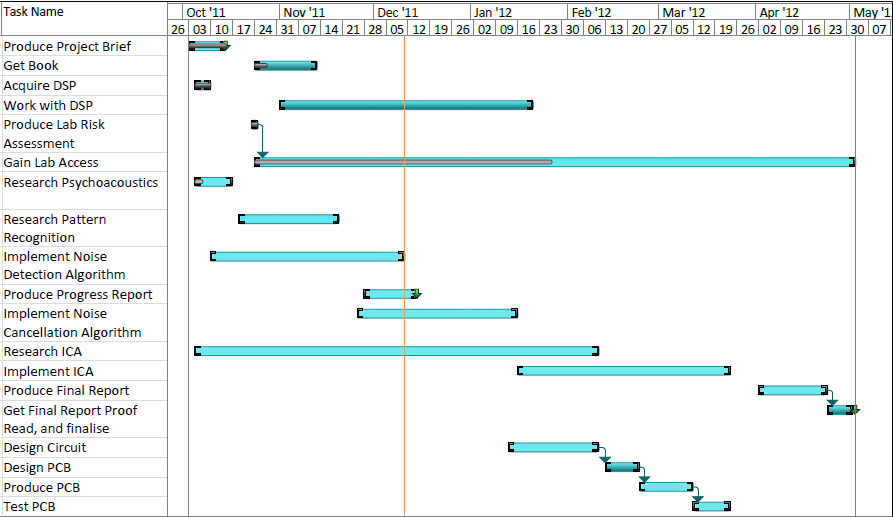
\includegraphics[width=\textwidth]{./img/ganntori.png}
	\caption{The Gannt chart for this project as originally produced}
	\label{fig:gannt}
\end{sidewaysfigure}

\noindent
The Gannt chart shown in figure~\ref{fig:gannt} changed regularly as time got reallocated and tasks got completed ahead or behind schedule.
By the end of the project, the Gannt chart stood as shown in figure \ref{fig:newgannt}.
\\
\begin{sidewaysfigure}
	\centering
	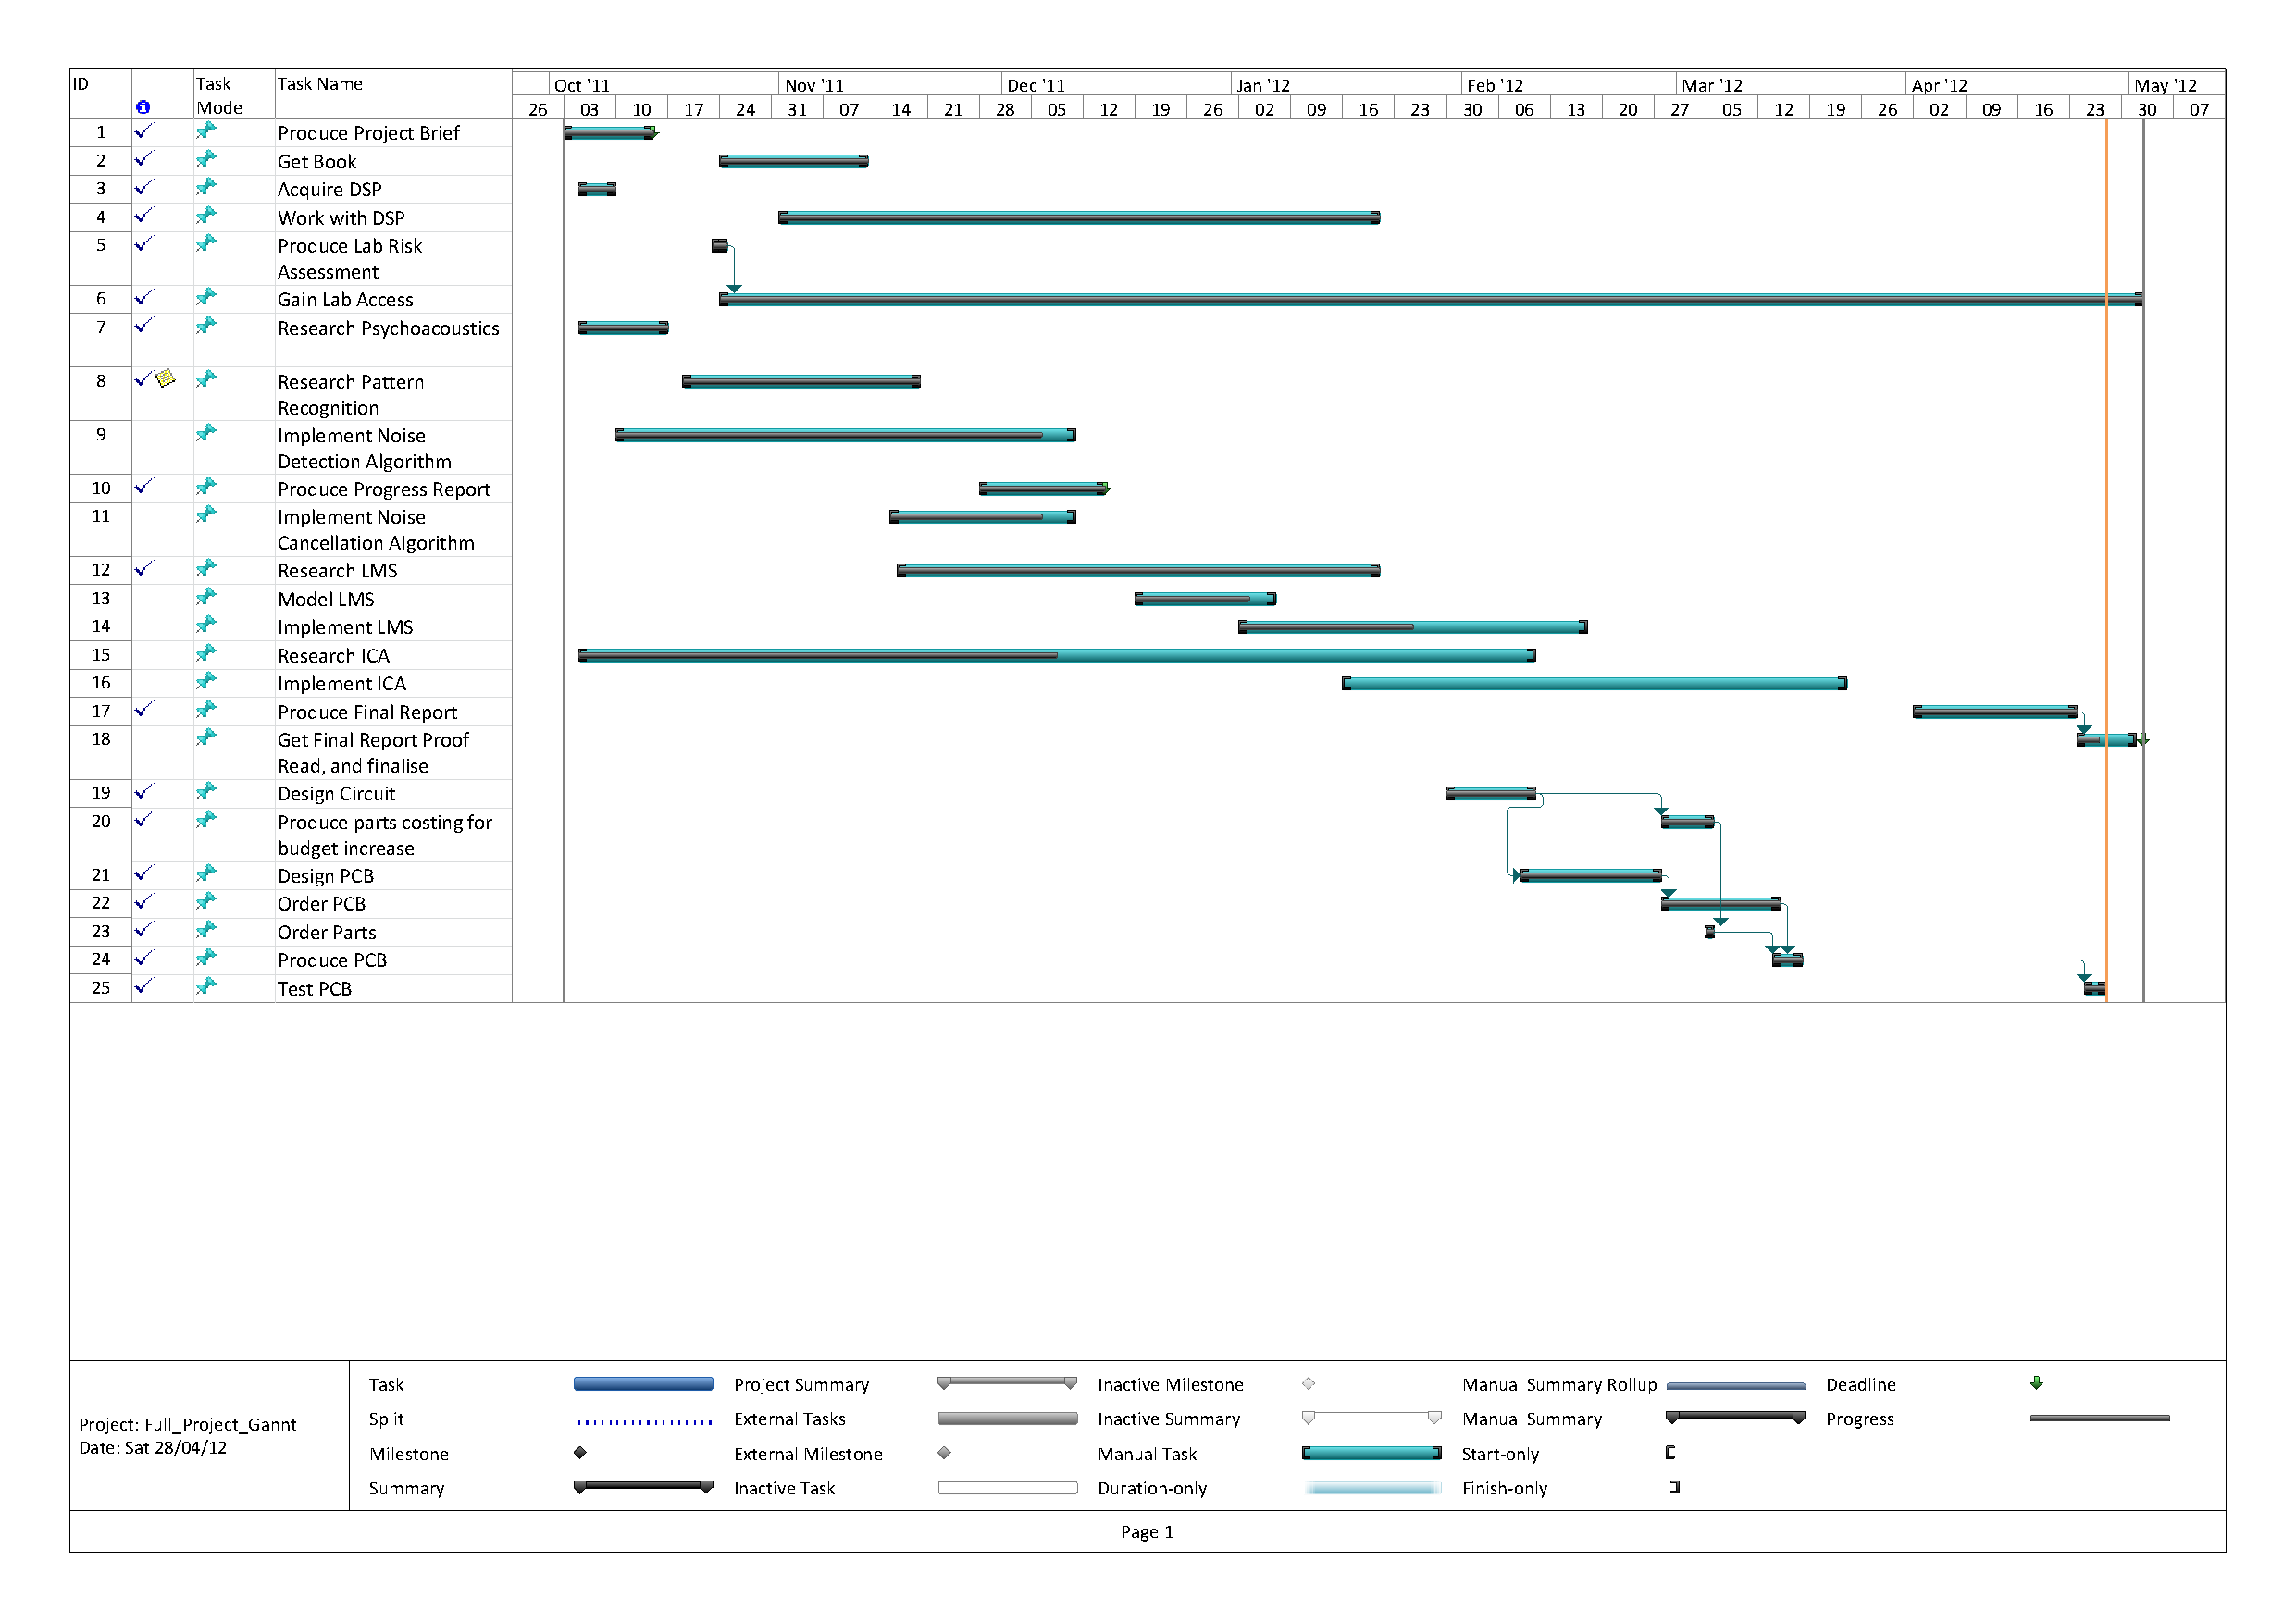
\includegraphics[width=\textwidth]{./img/Full_Project_Gannt_final.pdf}
	\caption{The Gannt chart for this project as of the progress report}
	\label{fig:newgannt}
\end{sidewaysfigure}

\noindent
A few differences can be seen between these two charts.
The majority of the differences are tasks that have been achieved, however it does show that some tasks ran behind schedule.
Another difference is the addition of some tasks, such as the production of costings to apply for a budget increase.
The general reason for tasks running behind schedule was due to problems in debugging, and not allowing suitable margins for fixing problems that arise.

\subsection{Weekly Tracker}
While Gannt Charts clearly show what should be being done and when, they are less representative of what should be being achieved in the short term.
As such the `Weekly Tracker' was developed in order to show what tasks needed to be achieved in the week, and to follow whether the project was on track on a weekly basis.
\\
\\
This is a sheet containing a list of tasks to be worked on during the coming week, including a review date on which the progress of each of these tasks would be noted and compared against the required progress.
\\
\\
Each task has a task name; also each task has space for notes at the beginning and end of the week.
Along with this, each task has a rank from 0 to 10 for minimum acceptable completion.
This is essentially the minimum percentage of the task that required to have been completed by the end of the week to remain on track.
Using a rank below 10 here allows for tasks to span multiple weeks, by increasing the required rank while progressing through the project.
There is also a rank for task completion.
This rank is out of the entire task, not just the amount required for the week, allowing progress beyond that expected for that week to be noted.
In the event of progression beyond the scope required by the overall task, this would be ranked as `+'.
At the end of the week on the review date, the sum of the differences between required and completed ranks would give a score for the week.
A negative score would denote that the project is behind schedule, whereas a positive score denotes that it is ahead of schedule.
A score of 0 indicating that it is on schedule.
An example of these can be seen in appendix \ref{appendix:weeklytracker}.
\\
\\
Table \ref{tab:scorings} shows the scores achieved on these weekly trackers.
\begin{table}[H]
	\centering
	\begin{tabular}[c]{| c | l | l | c |}
		\hline
		Sheet	& Start	& End	& Score \\
		\hline
		1	& 05/10/2011	& 09/10/2011	& -6	\\
		2	& 10/10/2011	& 16/10/2011	& -2	\\
		3	& 16/10/2011	& 23/10/2011	& -1	\\
		4	& 23/10/2011	& 30/10/2011	& -5	\\
		5	& 01/11/2011	& 06/11/2011	& -10	\\
		6	& 09/11/2011	& 13/11/2011	& -2	\\
		7	& 13/11/2011	& 20/11/2011	& -12	\\
		8	& 21/11/2011	& 27/11/2011	& -6	\\
		9	& 27/11/2011	& 04/12/2011	& -6	\\
		10	& 04/12/2011	& 11/12/2011	& 0	\\
		11	& 11/12/2011	& 18/12/2011	& -1	\\
		12	& 18/12/2011	& 08/01/2012	& -7	\\
		13	& 08/01/2012	& 29/01/2012	& -7	\\
		14	& 29/01/2012	& 05/02/2012	& -3	\\
		15	& 05/02/2012	& 12/02/2012	& 0	\\
		16	& 12/02/2012	& 19/02/2012	& -1	\\
		17	& 19/02/2012	& 26/02/2012	& -3	\\
		18	& 26/02/2012	& 04/03/2012	& 7	\\
		19	& 26/02/2012	& 04/03/2012	& 7	\\
		20	& 04/03/2012	& 11/03/2012	& -5	\\
		21	& 11/03/2012	& 18/03/2012	& -10	\\
		22	& 18/03/2012	& 01/04/2012	& -7	\\
		23	& 01/04/2012	& 15/04/2012	& -5	\\
		24	& 15/04/2012	& 22/04/2012	& 	\\
		\hline
	\end{tabular}
	\caption{Scorings of the weekly tracker}
	\label{tab:scorings}
\end{table}

\noindent These scorings show that the project was consistently behind schedule.
This was largely due to not fully anticipating how long certain aspects of the project would take, and unforeseen external factors.
Also the design of the weekly tracker doesn't particularly allow for scoring ahead of schedule.
This is because when work is completed significantly beyond the scope of the task an additional score of only 1 can be achieved, whereas negative scores are easier to achieve.


\subsection{Milestones}
In order to determine the state of the system, a collection of milestones has been set.
At each one the system would be able to demonstrate a level of functionality.
This would allow any major progress in the system to be noted and would allow the progress of the system to be observed.
Each milestone has a list of requirements which have to be met before it can be classed as achieved.
These milestones do not have to be met in the order stated, and some of them will be worked on in parallel, though in most cases the milestones build on the previous ones.

\begin{table}[H]
	\centering
	\begin{tabular}[c]{| c | l | c |}
		\hline
		No.	& Milestone		& Achieved? \\
		\hline
		1	& Record/replay audio	& X \\
		2	& Cancellation algorithm & X \\
		3	& Cancellation on DSP	& X \\
		4	& Create PCB		& \\
		5	& LMS algorithm		& \\
		6	& LMS on DSP		& \\
		7	& Add ICA		& \\
		\hline
	\end{tabular}
	\caption{The milestones set for the project}
	\label{tab:milestones}
\end{table}


\section{Correlation} 


\section{LMS}
LMS is a form of adaptive filter.
It works by reducing the average power of the feedback signal by modifying the coefficients in a Finite Impulse Response (FIR) filter.
An example implementation is shown below in figure~\ref{fig:lmsfilter}.
In this implementation the LMS algorithm will be used as the block labelled ``Adaptation algorithm''.
This version also aims for a slightly different effect to the method that will be employed in this project.
This project will be feeding the inverse of the noise estimate, -\^{n}(m), to the listener in order to generate the cancelling in their ear, rather than to remove the noise inside the software.

\begin{figure}[H]
	\centering
	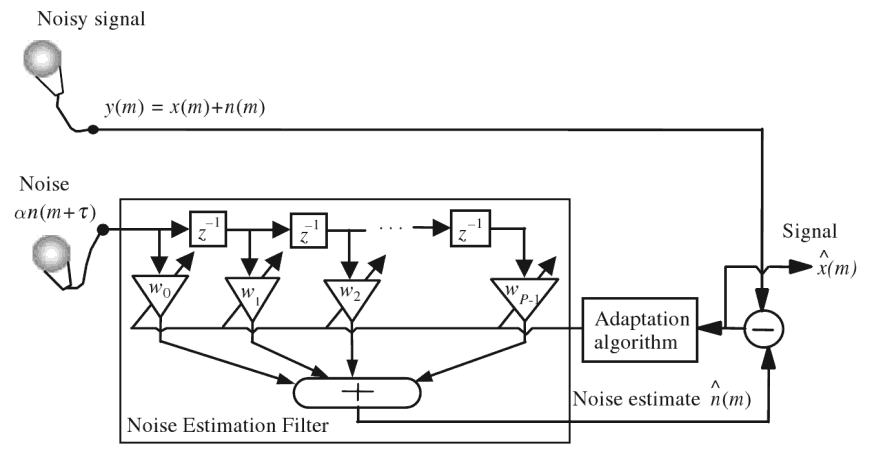
\includegraphics[width=\textwidth]{./img/lmsfilter.png}
	\caption{An example setup for the use of an LMS filter in noise cancellation (Sourced from Advanced Digital Signal Processing and Noise Reduction \cite{AdvancedDSPing})}
	\label{fig:lmsfilter}
\end{figure}




\section{PCB}

Along with the algorithmic side of the project, the hardware on which the algorithm would run was designed and produced.
This was produced in the form of a Printed Circuit Board (PCB) upon which would be placed the circuitry to run the various algorithms.
The necessary supporting electronics also had to be located on this PCB.
\\
\\
Due to the nature under which the system would be used, various features were required from the PCB.
Most significant the PCB had to be portable.
Headphones are generally used in circumstances where the users are moving about, sometimes in high risk circumstances.
As such the electronics on the PCB must not have interfered with the users' actions.
\\
\\
For starters, the PCB had to be compact.
Ideally, it should be of a size capable of fitting comfortably into a small pocket.
This would help prevent the system from mechanically interfering with the user.
Another aspect in which the PCB was designed so as not to impede the user was the power consumption.
The system had to be low power - capable of being powered by battery for an extended period of time.
This would allow the user to be mobile.


\newpage
\section{DSP vs. FPGA}
A DSP is not the only device that would be capable of supporting the processes required. One example of an alternative device is a Field-Programmable Gate Array (FPGA).

Notes:

DSP over FPGA:
\begin{itemize}
\item Larger memory for chip size (RAM would swallow basically entire chip)
\item Greater flexibility while programming (no hardware size limitations)
\item Pinout fixed, on reprogramming FPGA might want to change to make it physically possible, whereas DSP is fixed pinout and only code changes
\end{itemize}

FPGA over DSP:
\begin{itemize}
\item Potentially faster
\item More flexible for speed considerations (can implement multiple functions at once, while DSP can only do single instruction at a time)
\end{itemize}


\chapter{Modelling}
\section{Matlab}
In order to aid the design of the algorithms matlab models were produced and
tested.


\section{Hardware}
Much of the hardware used in this project is not possible to simulate, due to
the nature of the integrated circuits involved.
However, one aspect that can be simulated is the analogue circuitry before the
codec.

\subsection{Signal Conditioning}
Models of the signal conditioning were created in OrCAD in order to check that
the break frequency and roll off were suitable.
The design of this circuitry will be discussed later, in section
\ref{sec:imple:hard:sch} - only the modelling of it will be covered here.
The result of this modelling can be seen in figure \ref{fig:sigcondmodel}.
\\
\\
This graph shows that the signal conditioning amplifier has a break frequency
of 19409Hz.
This is ideal for the function it will be providing, as it is just below the
boundary of human hearing, meaning that all audible frequencies will reach 
the codec for sampling, while frequencies that would produce aliasing are
nullified.

\begin{figure}[H]
	\centering
	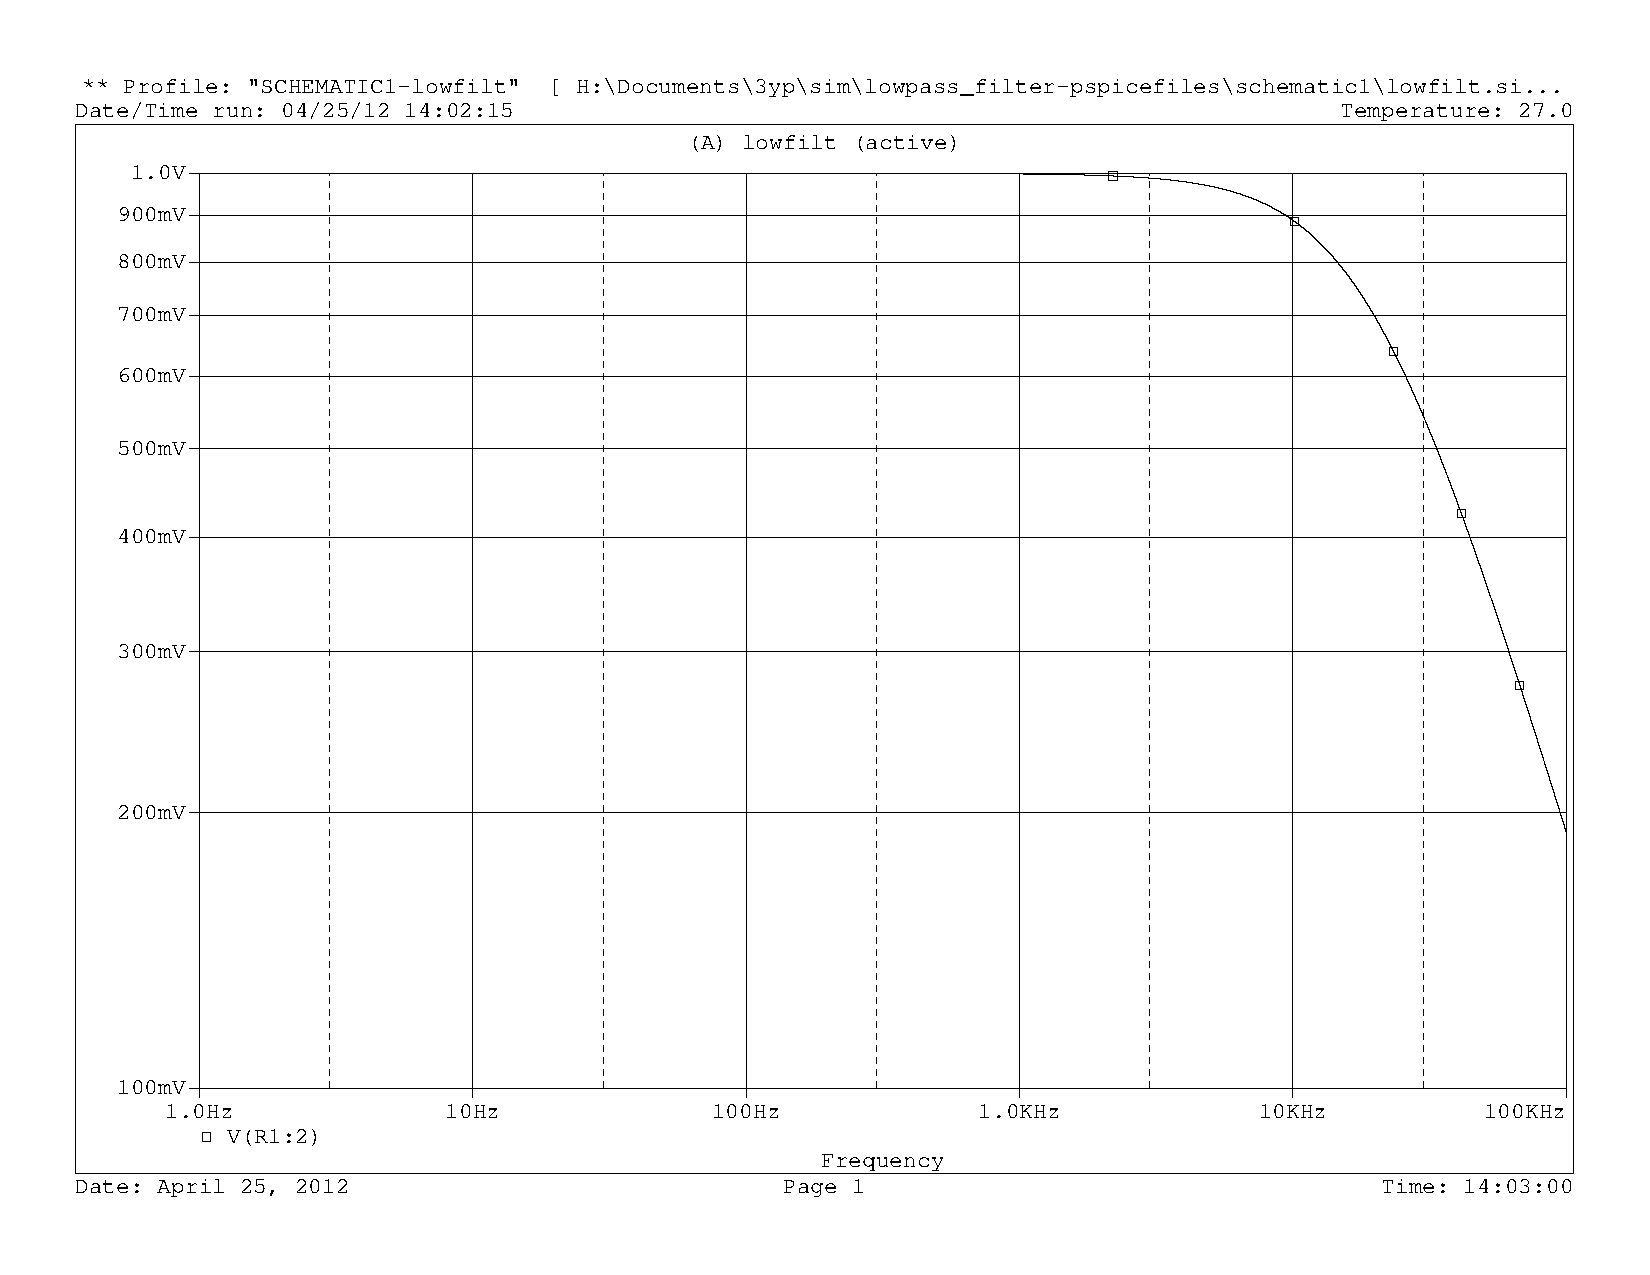
\includegraphics[width=\textwidth]{./img/signal_conditioning_sim.pdf}
	\caption{Simulation results of the signal conditioner}
	\label{fig:sigcondmodel}
\end{figure}

\subsection{Summing Amplifier}
A model of the summing (or instrumentation) amplifier was produced to check that it would function
as desired.
As the amplifier being used was not originally conceived for the use to which
it is put to in this project, modelling was even more important to check that
it would function as desired.
Although the produced amplifier would operate on two channels, as these channels
are identical, only one was simulated.

\begin{figure}[H]
	\centering
	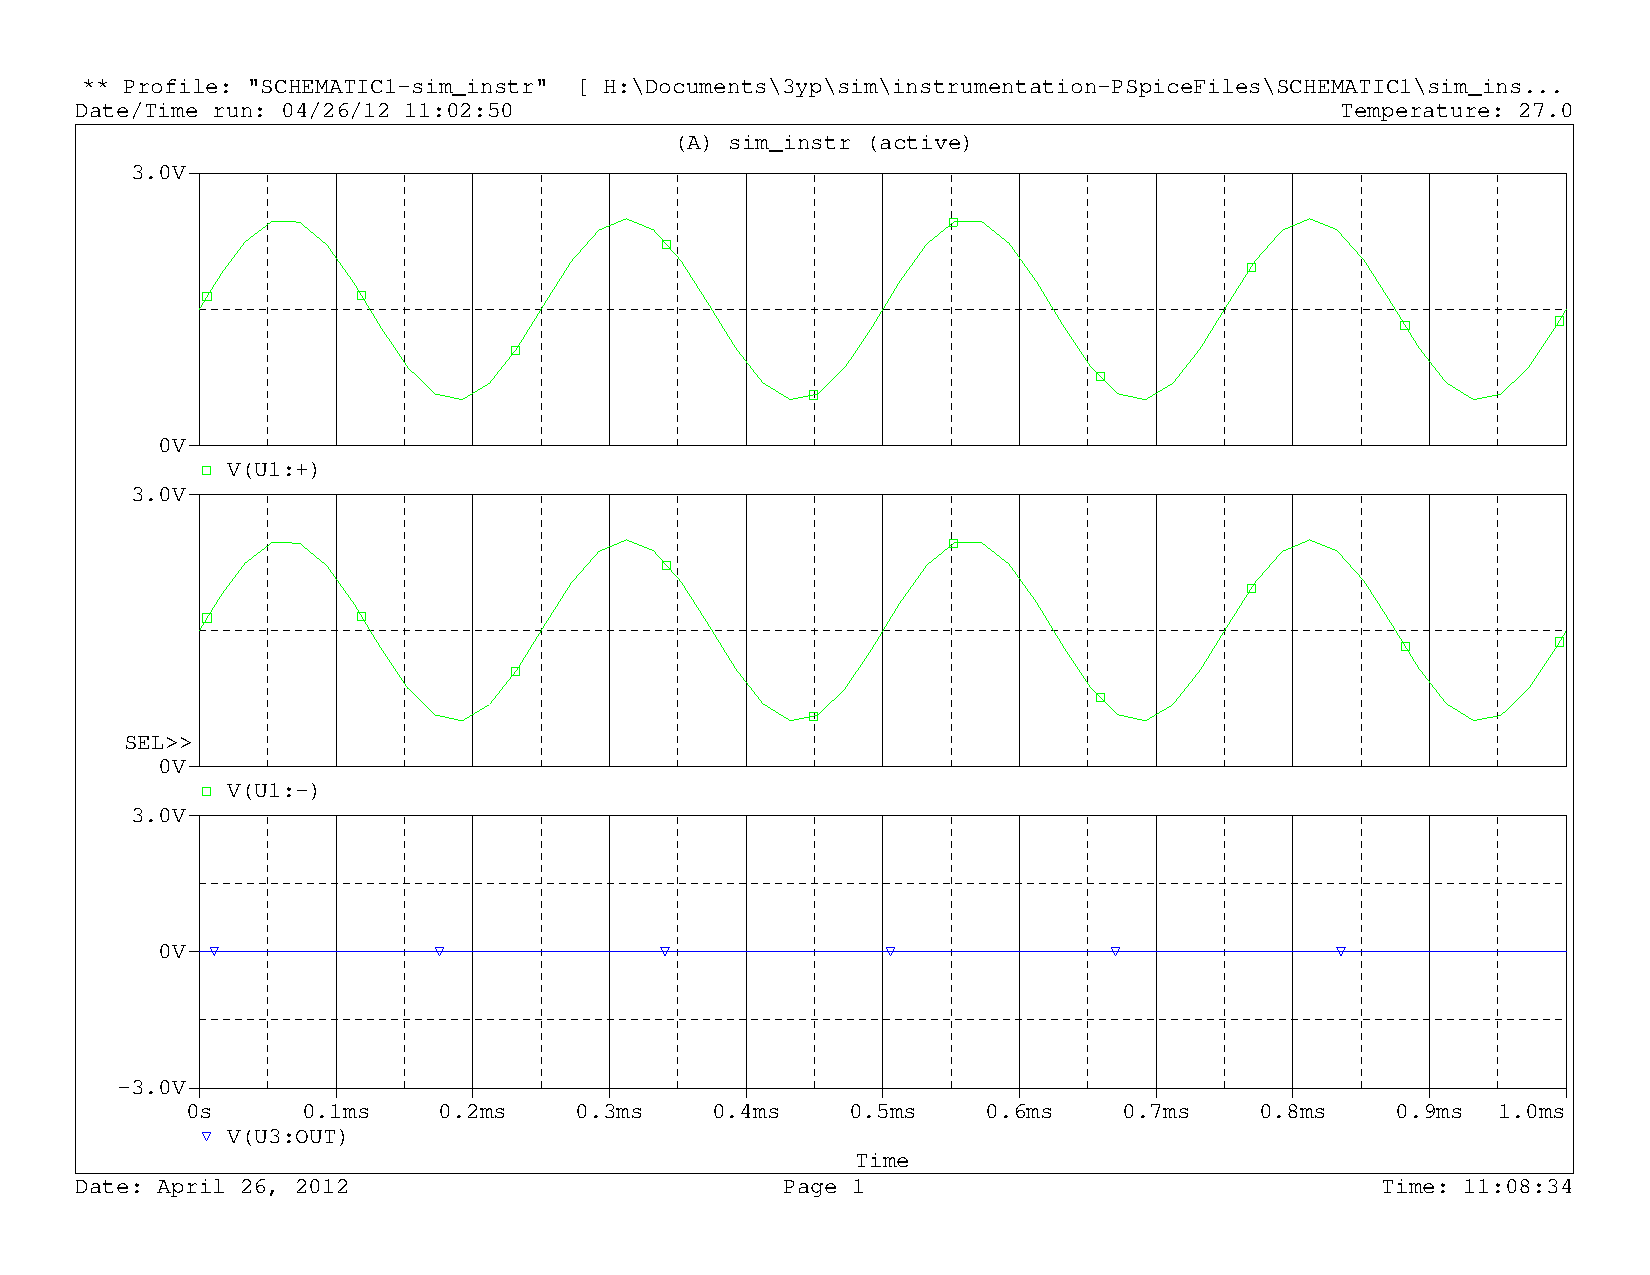
\includegraphics[width=\textwidth]{./img/instrumentationamp.pdf}
	\caption{The output from the instrumentation amplifier from two identical sine waves}
	\label{fig:instramp}
\end{figure}

\noindent Figures \ref{fig:instramp} and \ref{fig;instrampbeat} show that the summing amplifier will correctly sum the two signals together, with one of the signals experiencing a 180$^{\circ}$ phase shift.

\begin{figure}[H]
	\centering
	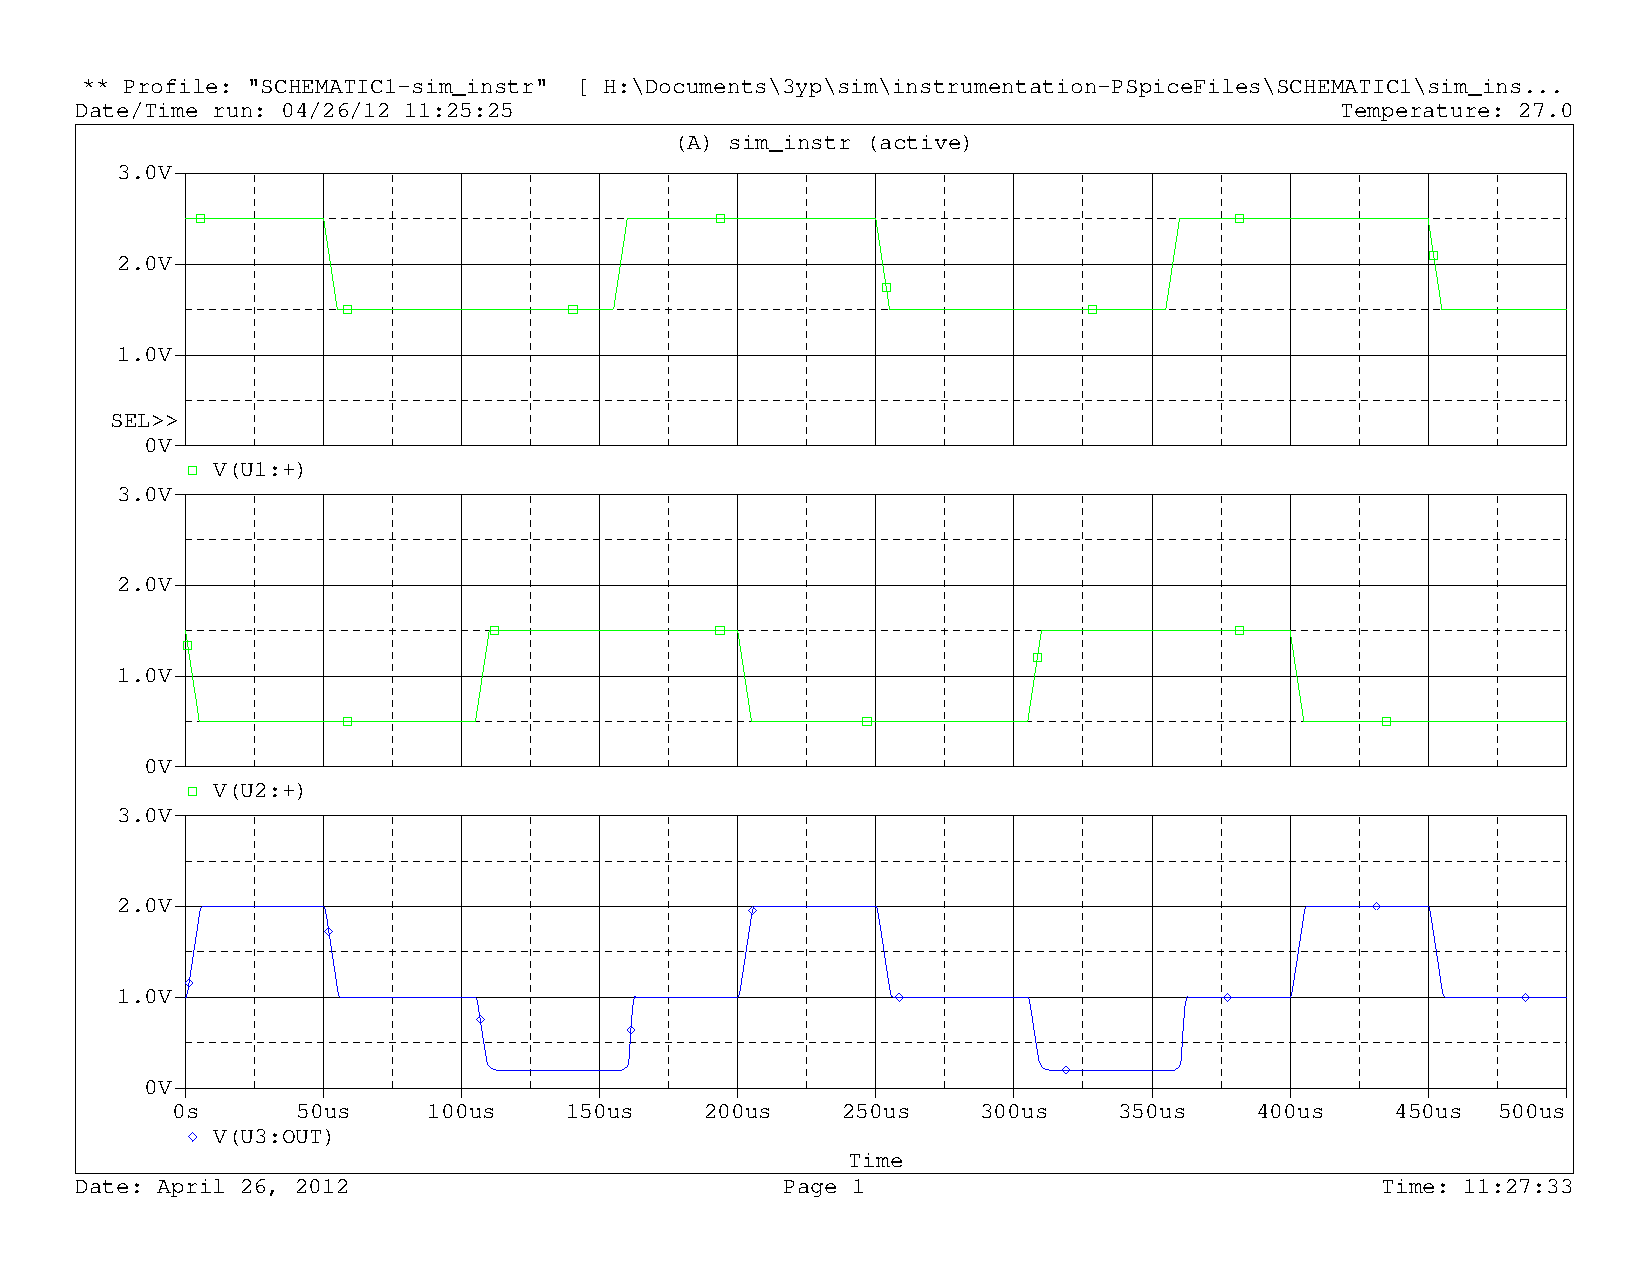
\includegraphics[width=\textwidth]{./img/instrumentationamp_dig.pdf}
	\caption{The output from the instrumentation amplifier from two digital signals}
	\label{fig:instrampbeat}
\end{figure}


\chapter{Implementation}

\section{Hardware}

There are two parts to this project, the software, algorithmic side of things, and the hardware on which this algorithm runs.
Here the details about the design and production of the PCB will be discussed, and explanations of why certain decisions were made.

\subsection{Schematic}
\label{sec:imple:hard:sch}
Before producing the PCB design the system was designed in gEDA Schematic software.
In order to keep the design easy to maintain hierarchy was used, and the system split into multiple sections.
These sections are discussed below.

\begin{figure}[H]
	\centering
	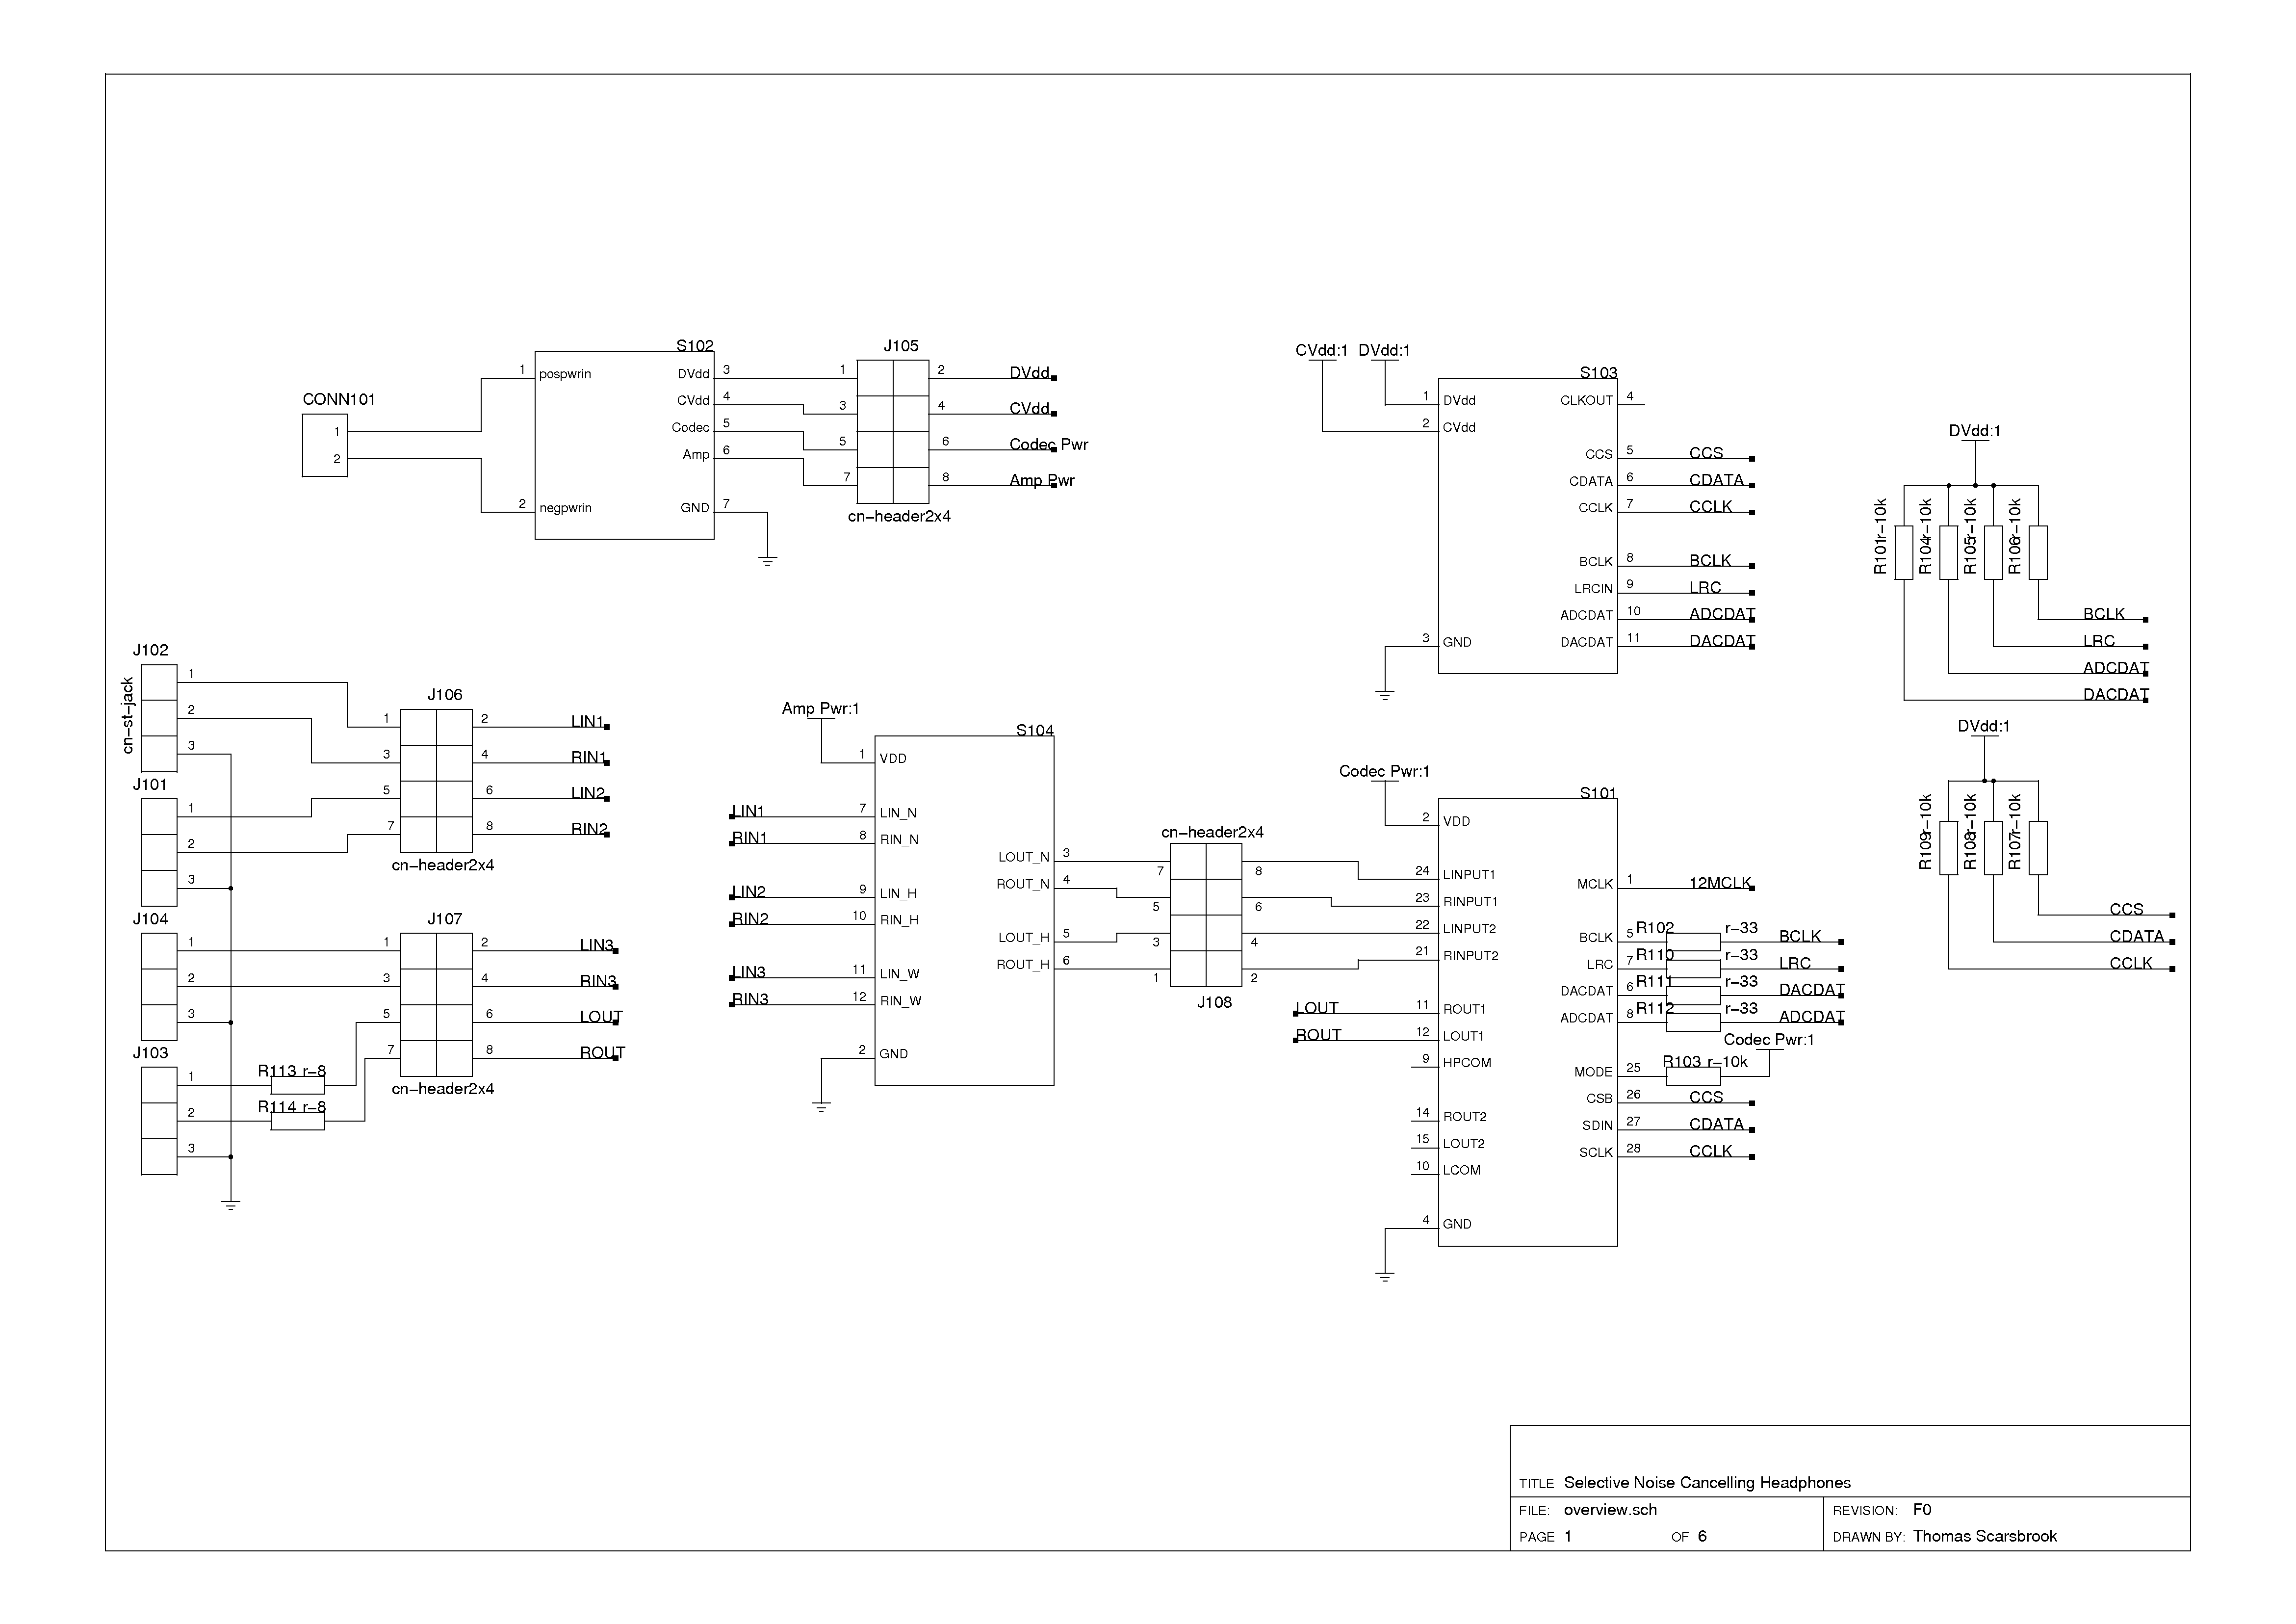
\includegraphics[width=\textwidth]{./img/overview.png}
	\caption{The top level schematic}
	\label{fig:overviewsch}
\end{figure}

\subsubsection{DSP}
At the heart of the project is the digital signal processor.
This is the part that achieves all the calculations required by the cancelling algorithm.
The DSP chosen for this project was the Texas Instruments TMS320C6713.
It was chosen as it had the desired interfaces required for communication with the codec, and was powerful enough to support the desired algorithms
Another important factor used in the decision was that a development board for this DSP could be acquired, allowing the testing of code without requiring the PCB being produced.
Due to the complexity of the design, the DSP required two separate voltage levels, one for the core logic and one for the I/O, and required connectivity to them at multiple points around the device.
A significant number of decoupling capacitors were required at these power connections, in order to prevent noise from disrupting correct operation.
These capacitors can be seen in figure \ref{fig:dspdecouplingcaps}.

\begin{figure}[H]
	\centering
	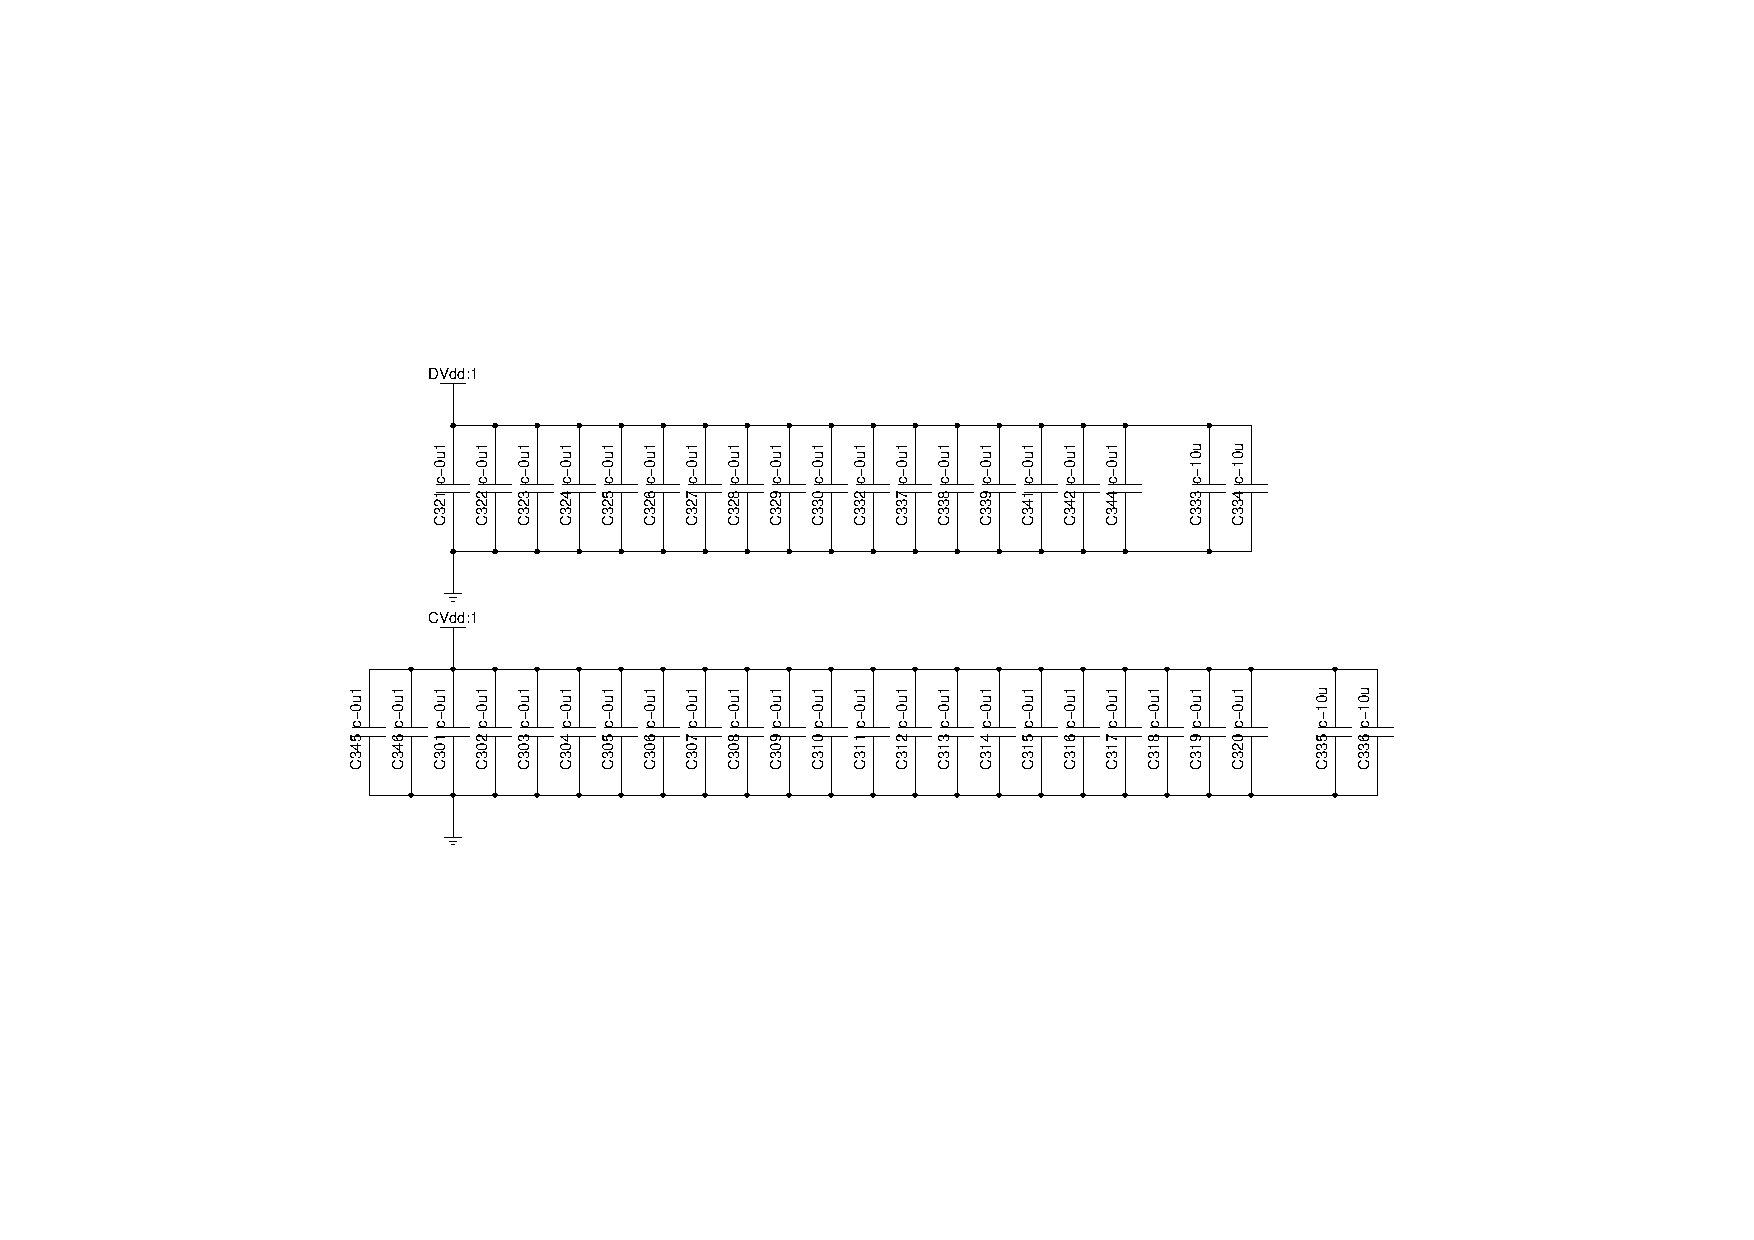
\includegraphics[width=\textwidth]{./img/dsp_decoupling.pdf}
	\caption{Decoupling capacitors for the DSP}
	\label{fig:dspdecouplingcaps}
\end{figure}

\noindent It is rather difficult to tell how code is operating on a DSP, due to the fact that the internals cannot be probed.
This becomes harder when debugging, as the code could be causing the DSP to crash.
If this were to happen then it has the potential to cause any debugging software to crash also, preventing the use of a stack trace.
As a way to circumvent this issue, a couple of LEDs were added to the DSP, connected to the general purpose I/O pins.
These could then be used for debugging, and potentially to display details to the user in a final product.

\begin{figure}[H]
	\centering
	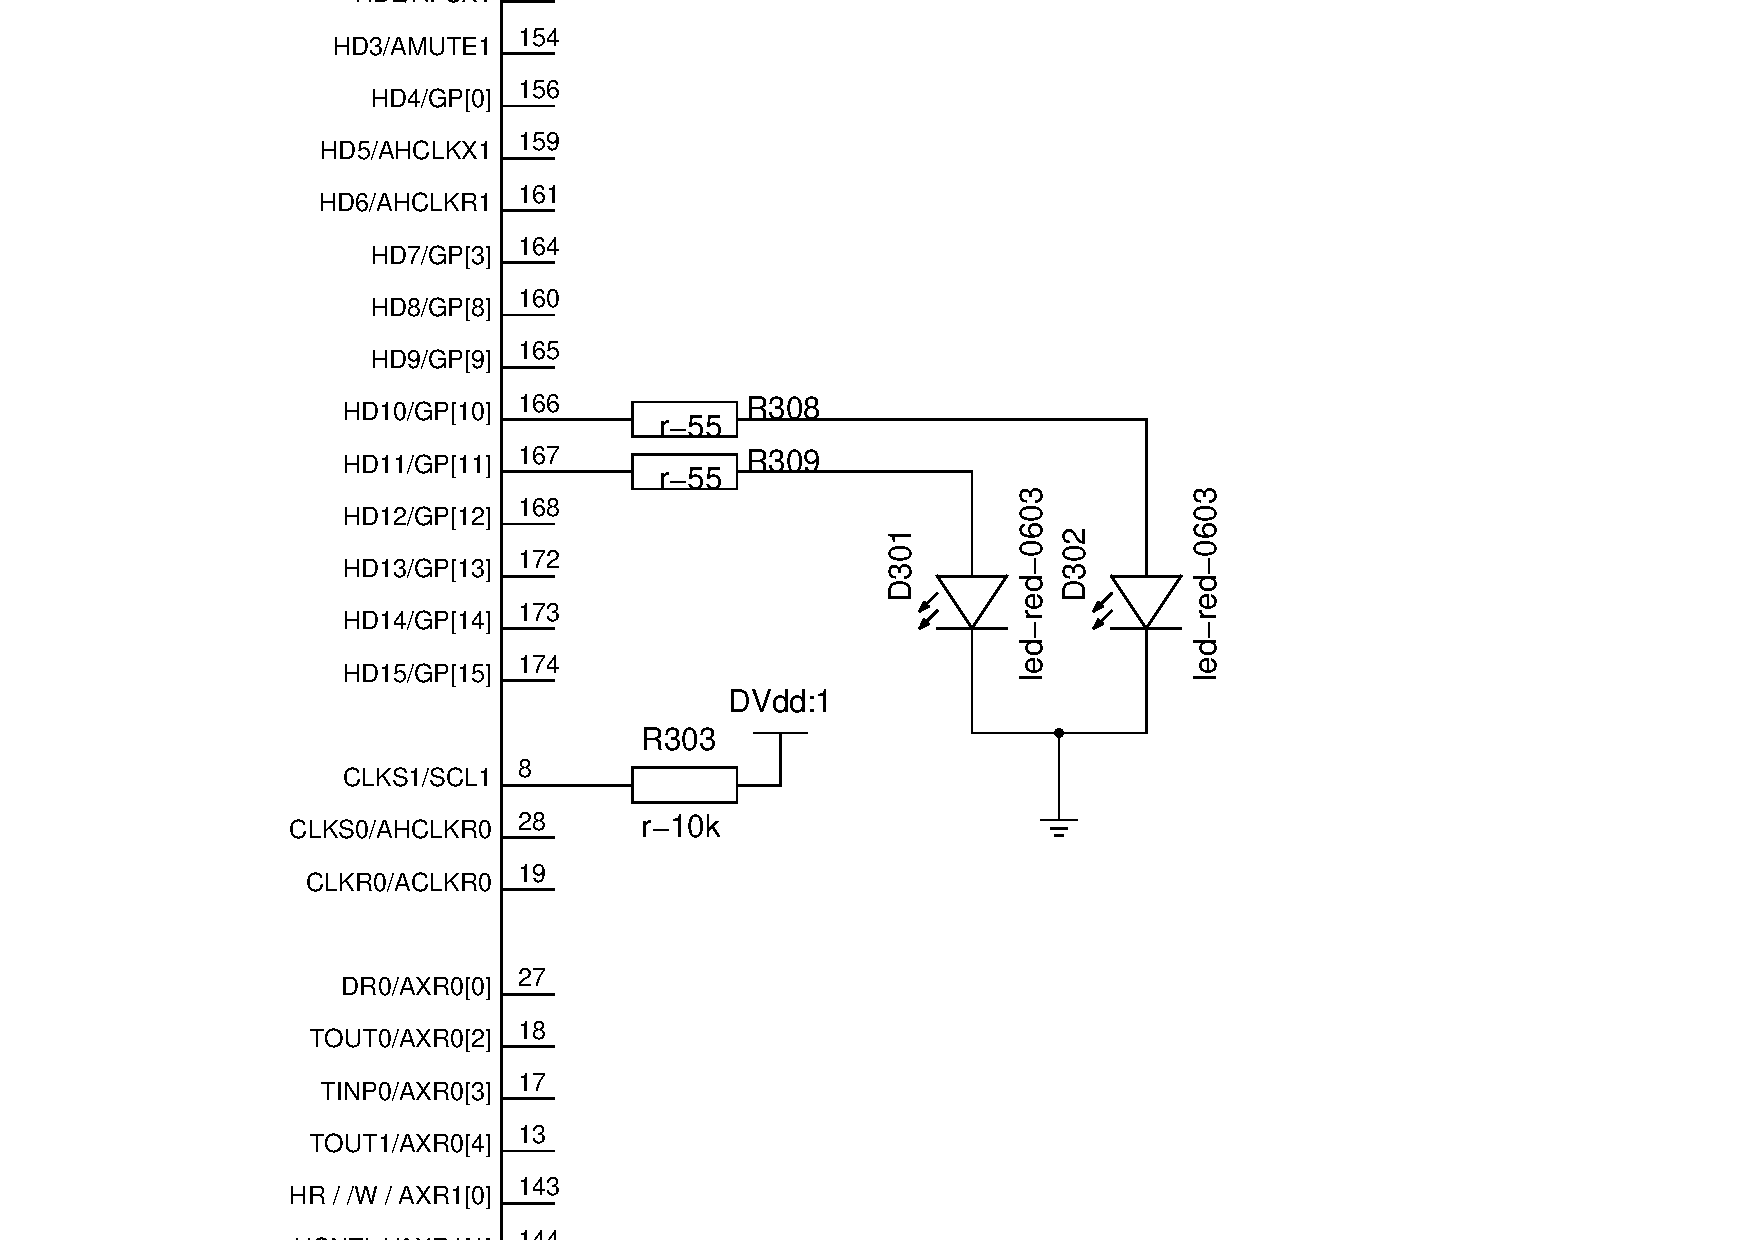
\includegraphics[width=\textwidth]{./img/dsp_LEDs.pdf}
	\caption{Debugging LEDs for the DSP}
	\label{fig:dspdebugleds}
\end{figure}

\noindent In order to program and debug the DSP a JTAG header was set up.
The header used was compatible with the standard Texas Instruments 14 pin JTAG connector, to enable use of standard programming tools.
The pin layout for this header can be seen in table \ref{tab:jtagpinout}.

\begin{table}[H]
	\centering
	\begin{tabular}[c]{| c | l |}
		\hline
		Pin	& Function	\\
		\hline
		1	& TMS		\\
		2	& nTRST		\\
		3	& TDI		\\
		4	& GND		\\
		5	& $DV_{dd}$	\\
		6	& KEY		\\
		7	& TDO		\\
		8	& GND		\\
		9	& RTCK		\\
		10	& GND		\\
		11	& TCK		\\
		12	& GND		\\
		13	& EMU0		\\
		14	& EMU1		\\
		\hline
	\end{tabular}
	\caption{JTAG pin assignments used}
	\label{tab:jtagpinout}
\end{table}

\subsubsection{Codec}
The DSP is unable to read analogue signals, and therefore requires the analogue signals from the microphones involved to be sampled by an external device.
This is where the codec comes in.
Wolfson MicroElectronics WM8988 was chosen for four reasons.
Firstly it supports a communication protocol supported by the McBSP system on the DSP.
This allows the configuration of the codec to be set easily, along with the acquisition and outputting of audio samples.
Secondly the codec provides two stereo inputs, which is what is required for this project, one for the noise signal, one for the heard/demanded signal.
On top of this the codec has a output with a headphone driver, meaning that no further electronics is required between the codec and the headphones, so impedance matching is not an issue.
Finally, the codec supported sampling frequencies suitable for the full spectrum of human hearing, meaning high frequency components would not evade being cancelled.
\\
\\
However, the codec could not function purely by itself, it requires some surrounding electronics.
Some basic resistors and capacitors are required on the codecs I/O ports, but the most significant piece of supporting electronics it required was a clock.
This clock was required so it could generate the appropriate timings for the sampling frequencies and the communications with the DSP.

\begin{figure}[H]
	\centering
	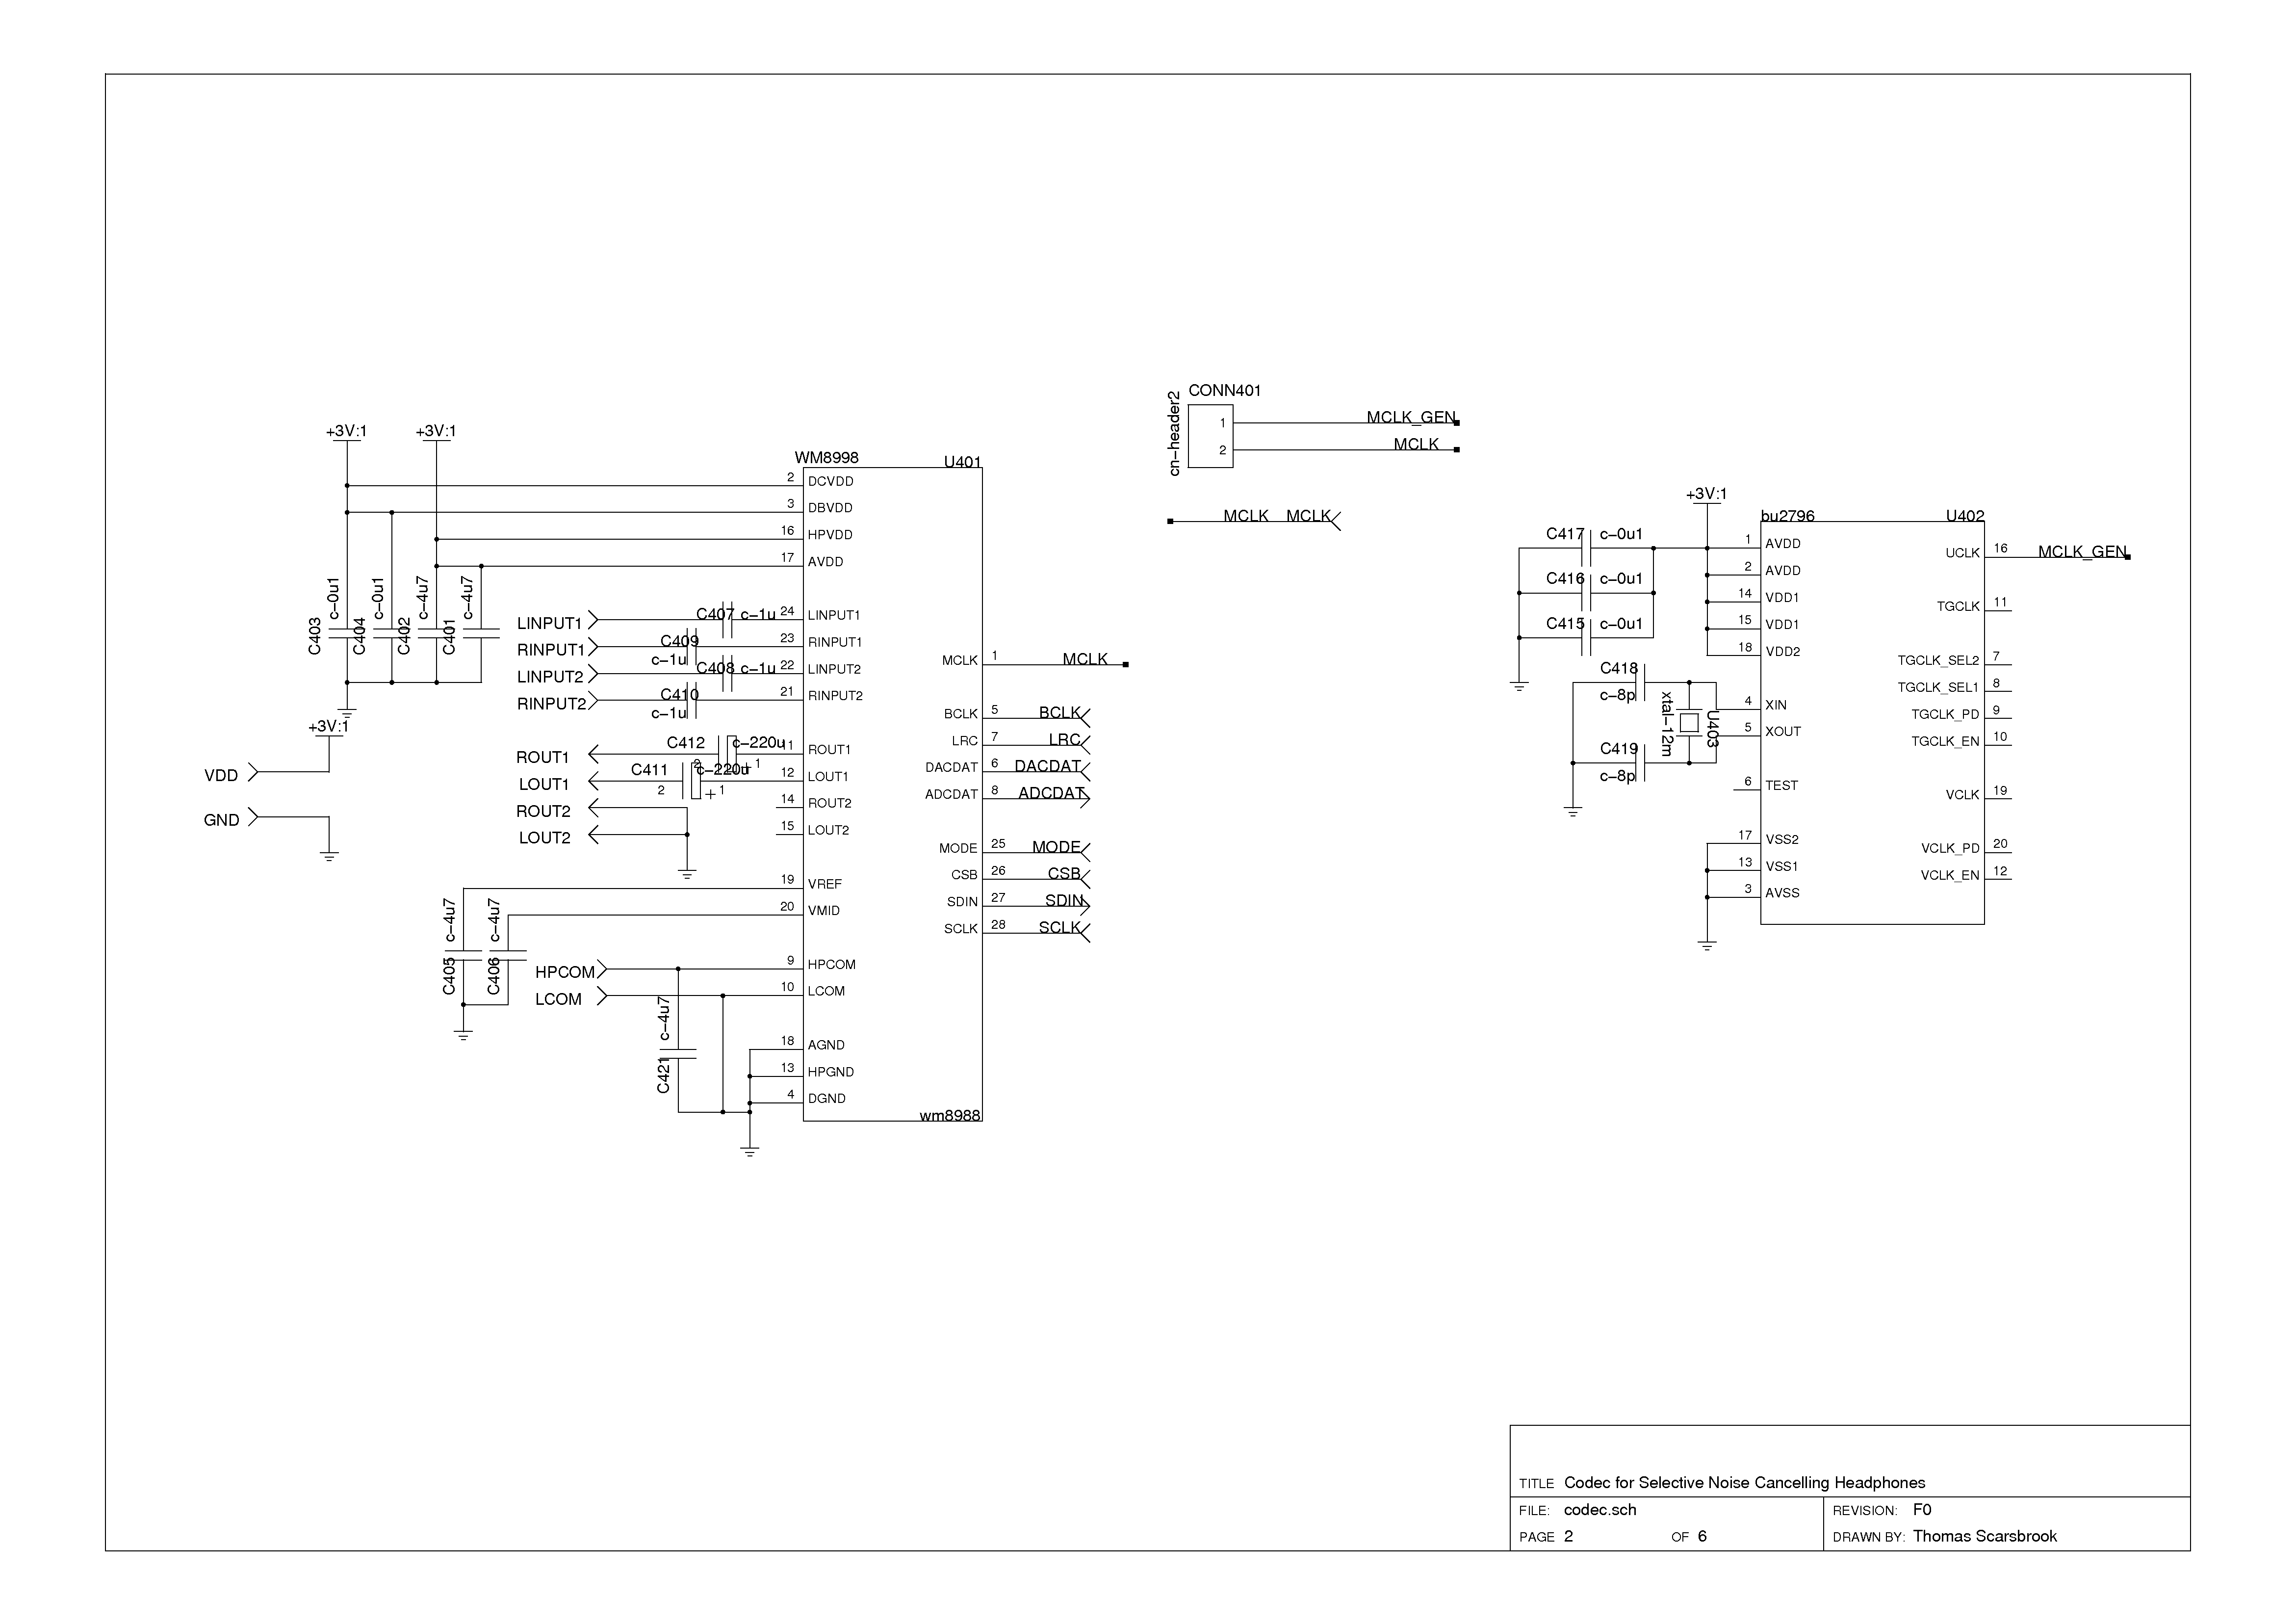
\includegraphics[width=\textwidth]{./img/codec.png}
	\caption{The schematic for the codec}
	\label{fig:codecsch}
\end{figure}

\subsubsection{Analogue}
Before the codec the signal needs some conditioning.
If any signal received were to be passed into the codec it could contain components at too high a frequency, these need to be removed to prevent aliasing.

\begin{figure}[H]
	\centering
	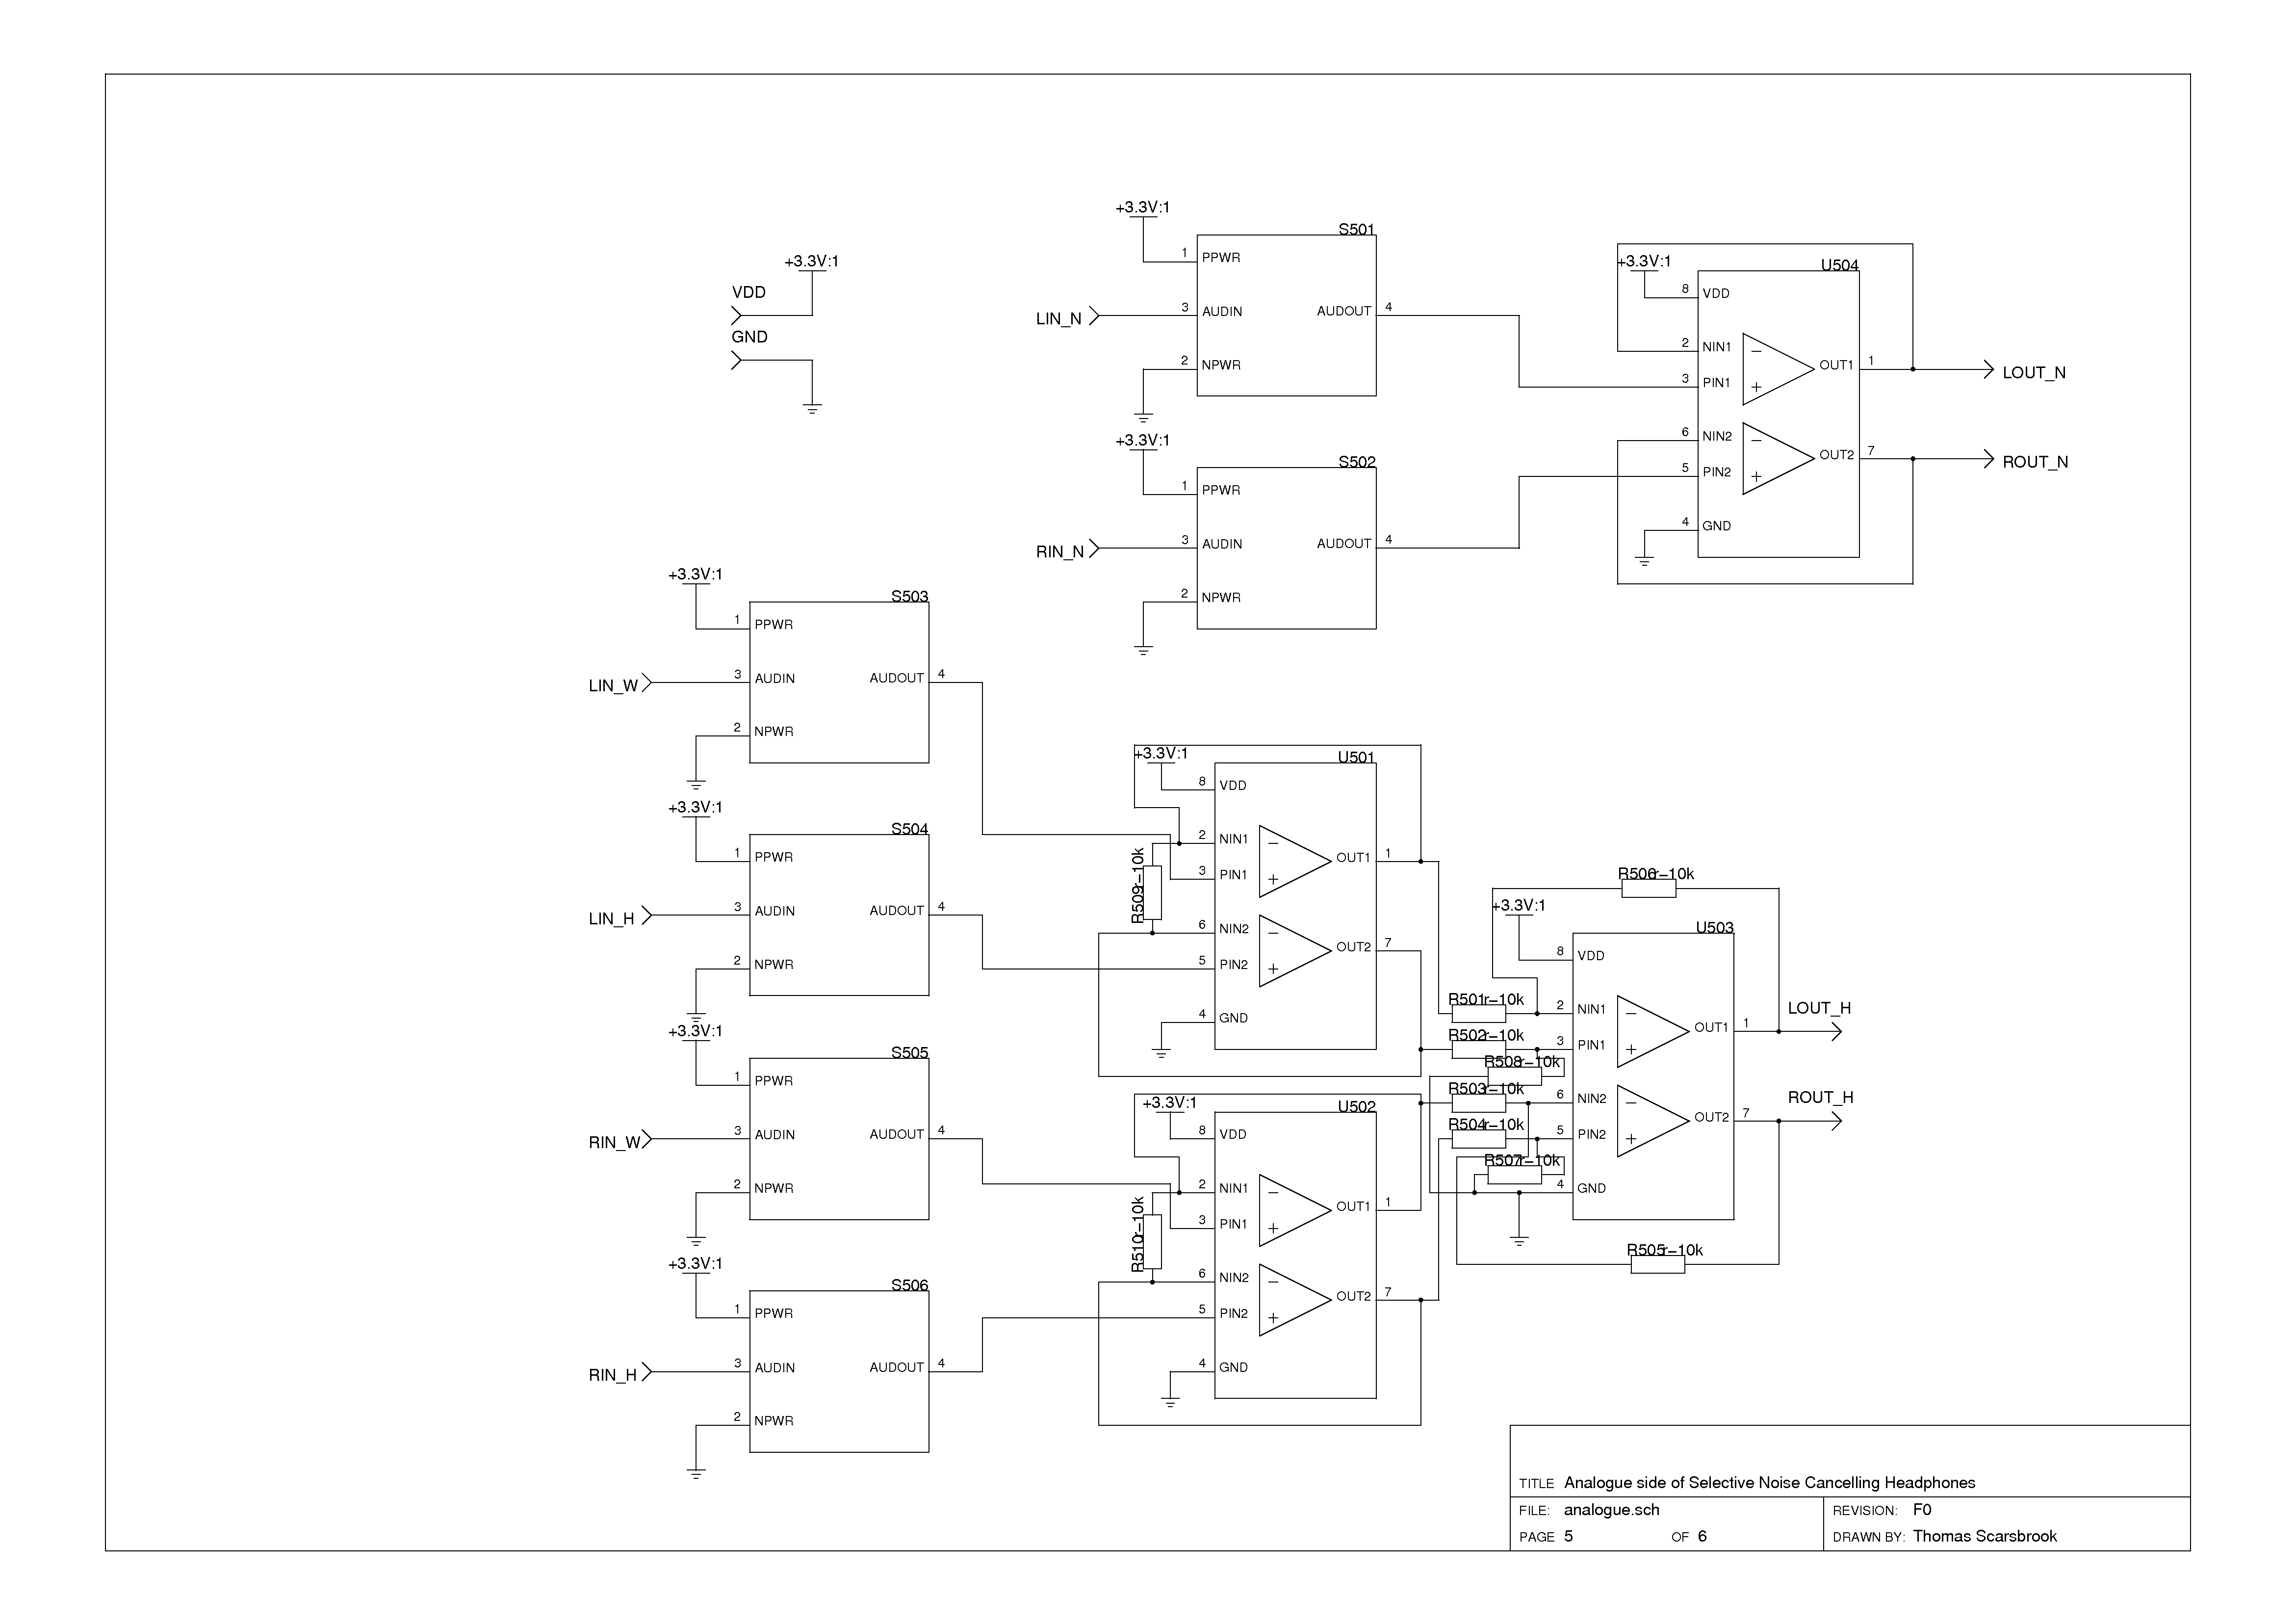
\includegraphics[width=\textwidth]{./img/analogue.png}
	\caption{The schematic of the analogue portion of the project}
	\label{fig:analoguesch}
\end{figure}

\noindent This portion of the design is then further split into two parts, the instrumentation amplifier and the signal conditioning.
The instrumentation amplifier takes in the noise and the optional demanded signal, and sums the two together.
This choice of amplifier was based on a few requirements.
The inputs from the microphones on the headphones require the amplifier to have a large input impedance.
Using a naive summing amplifier would result in a much lower input impedance due to the mixing resistors.
In contrast, the demanded input is likely to be from an MP3 player or similar, which will provide a low output impedance due to being designed to connect direct to, and drive headphones.
As such this input does not require the same high impedance from the amplifier, however the signal is not harmed by it.
Providing this high impedance also allows microphones to be connected and still serve equally well.
The second requirement of the amplifier is that it must sum the signals together with minimal distortion to the heard signal.
Adding distortion would result in sub-optimal cancellation, due to the actual heard signal not being known.
The instrumentation amplifier is a difference amplifier, as such one of its input is affected by a phase shift of 180$^{\circ}$.
As the demanded signal has no specific requirement for phase being maintained, this signal is the one that gets inverted.
\\
\\
Signal conditioning is required in order to prevent aliasing occurring when the input signals are sampled.
In order to accomplish this a naive low-pass filter was used, as shown in figure \ref{fig:sigcondsch}.
This design was chosen due to its simplicity to implement and minimal power draw, whilst still maintaining a high input impedance and suitable roll-off.

\begin{figure}[H]
	\centering
	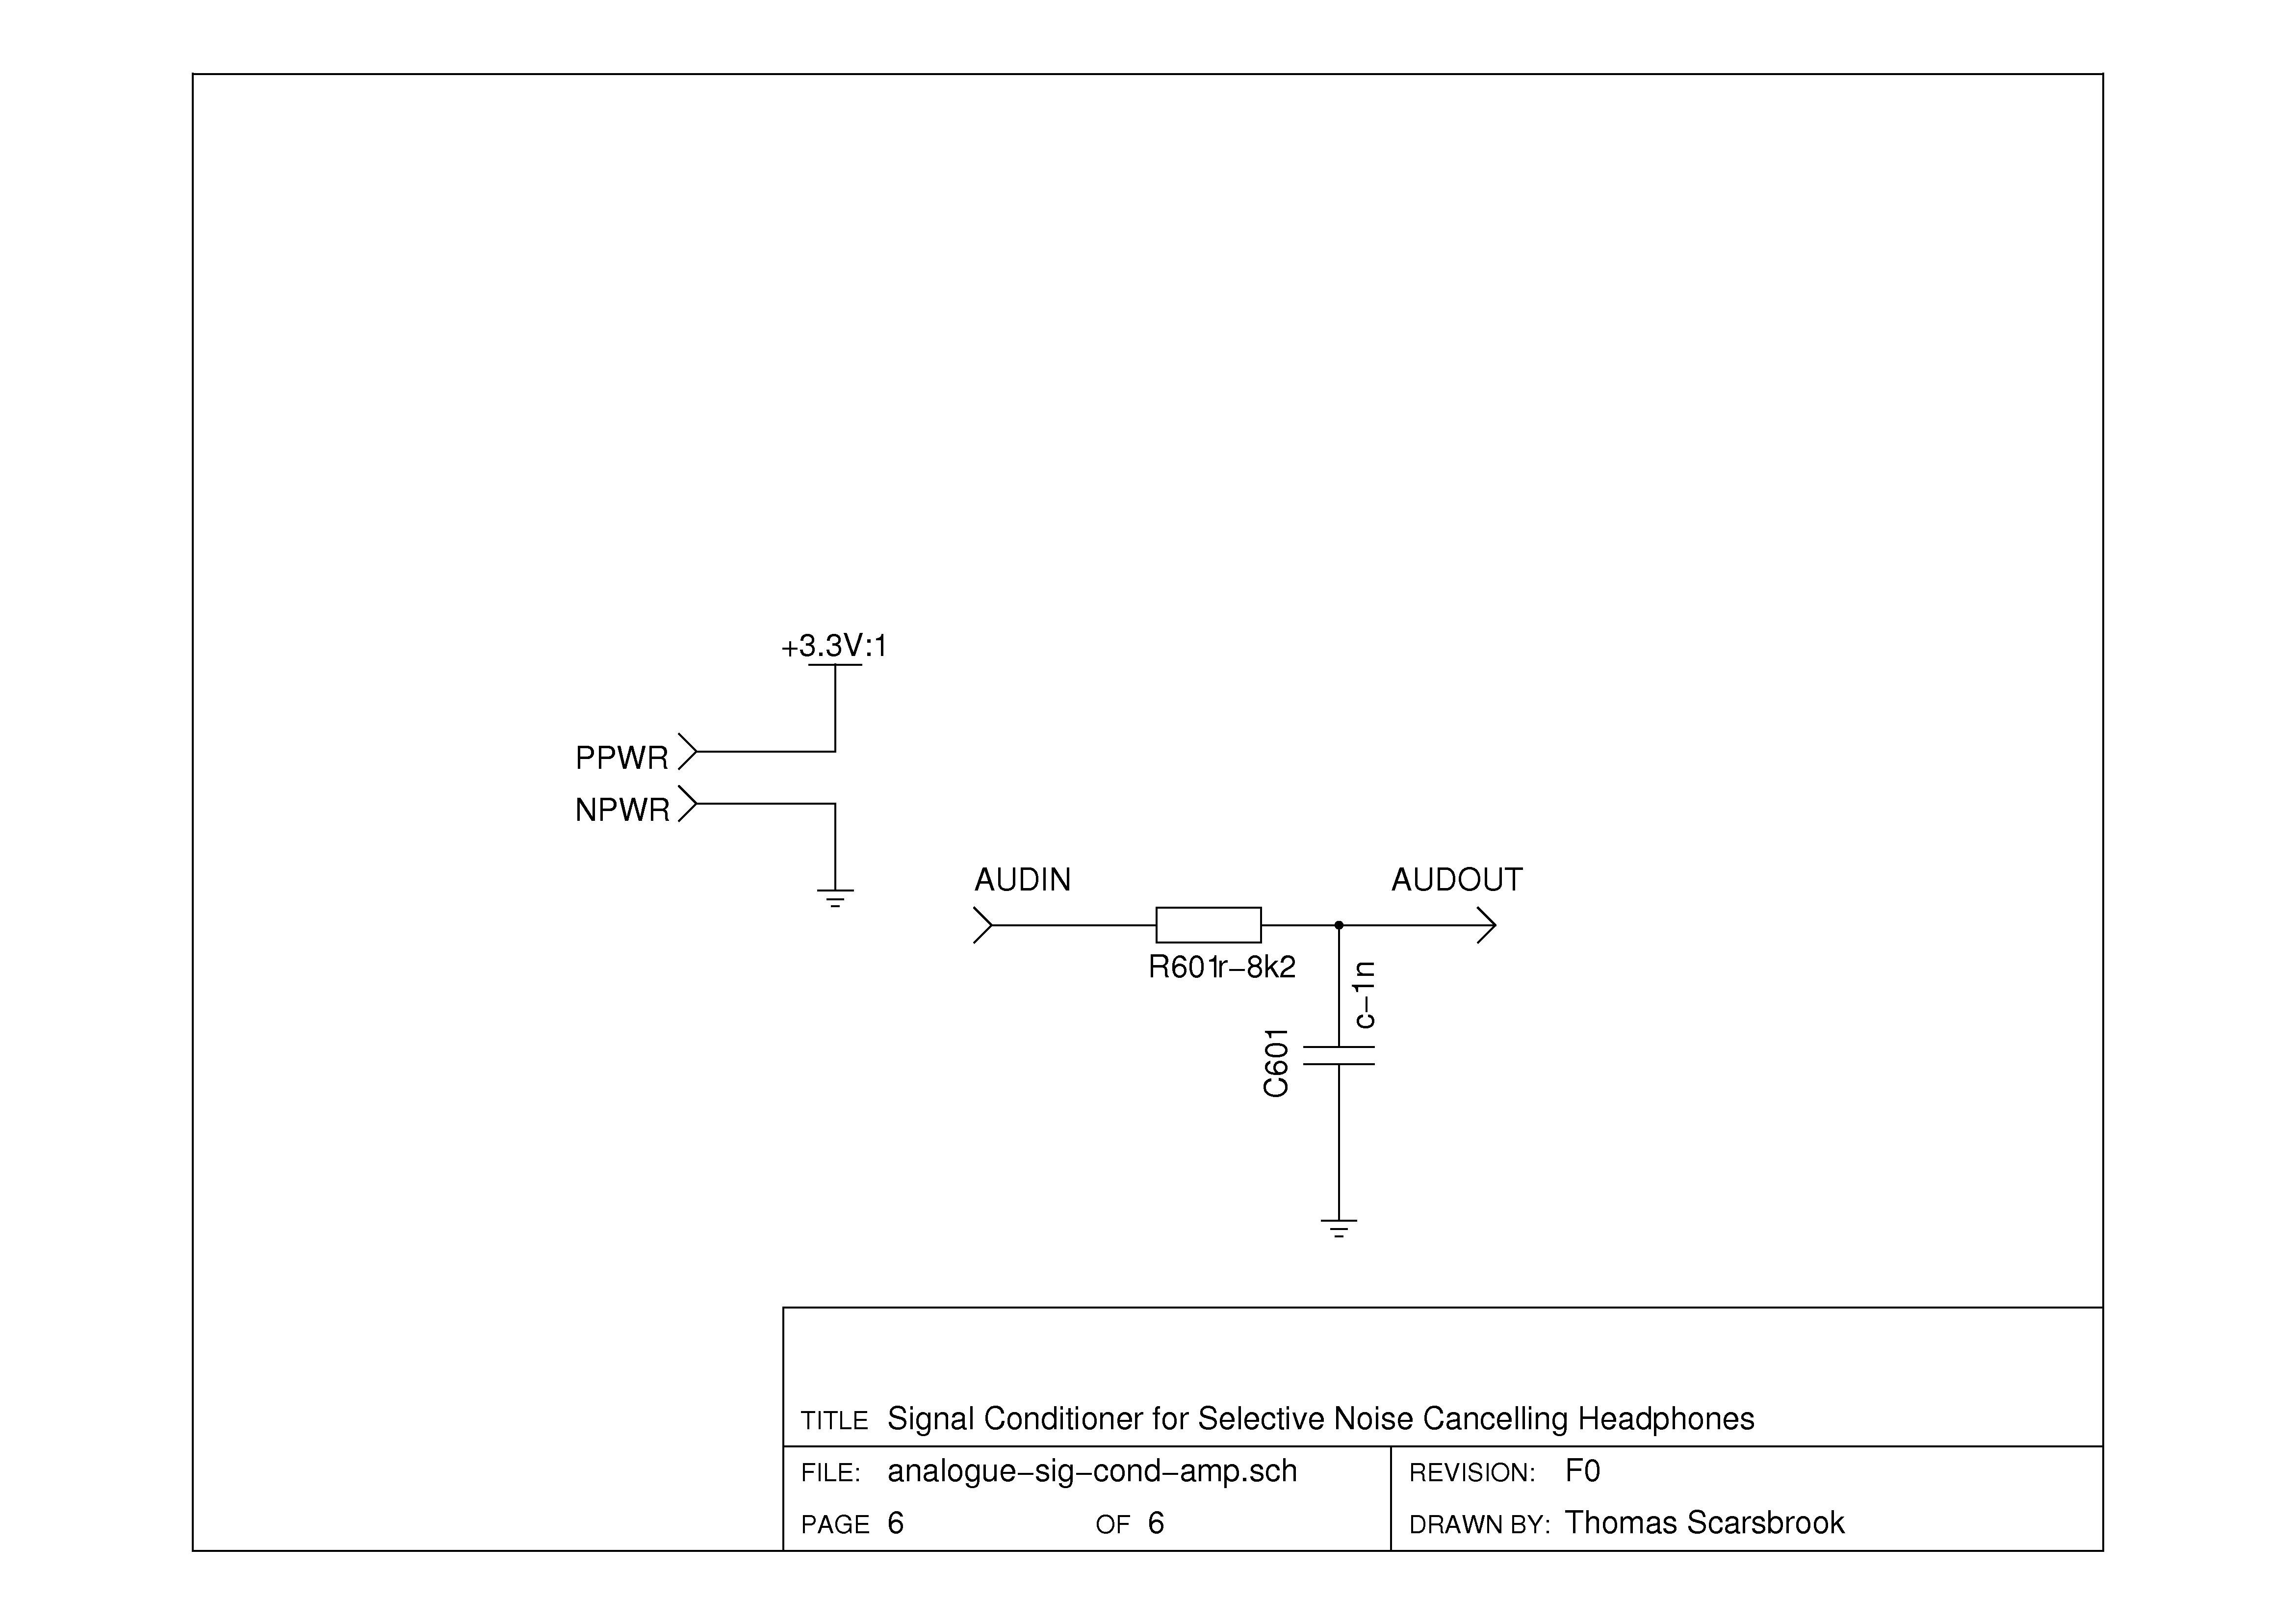
\includegraphics[width=\textwidth]{./img/analogue-sig-cond-amp.png}
	\caption{The signal conditioning amplifier schematic}
	\label{fig:sigcondsch}
\end{figure}

\noindent This design was tested through the use of a signal generator and digital oscilloscope.
The results can be seen below.

\subsubsection{Power}
One key part of any electronic system is it needs some form of power supply, and this project is no exception.
Multiple voltage rails were required, due to the DSP requiring a core voltage level as well as a second level for I/O.
The voltage level required by the codec and the amplifiers was the same as the one required by the DSP I/O, simplifying the design.

\begin{figure}[H]
	\centering
	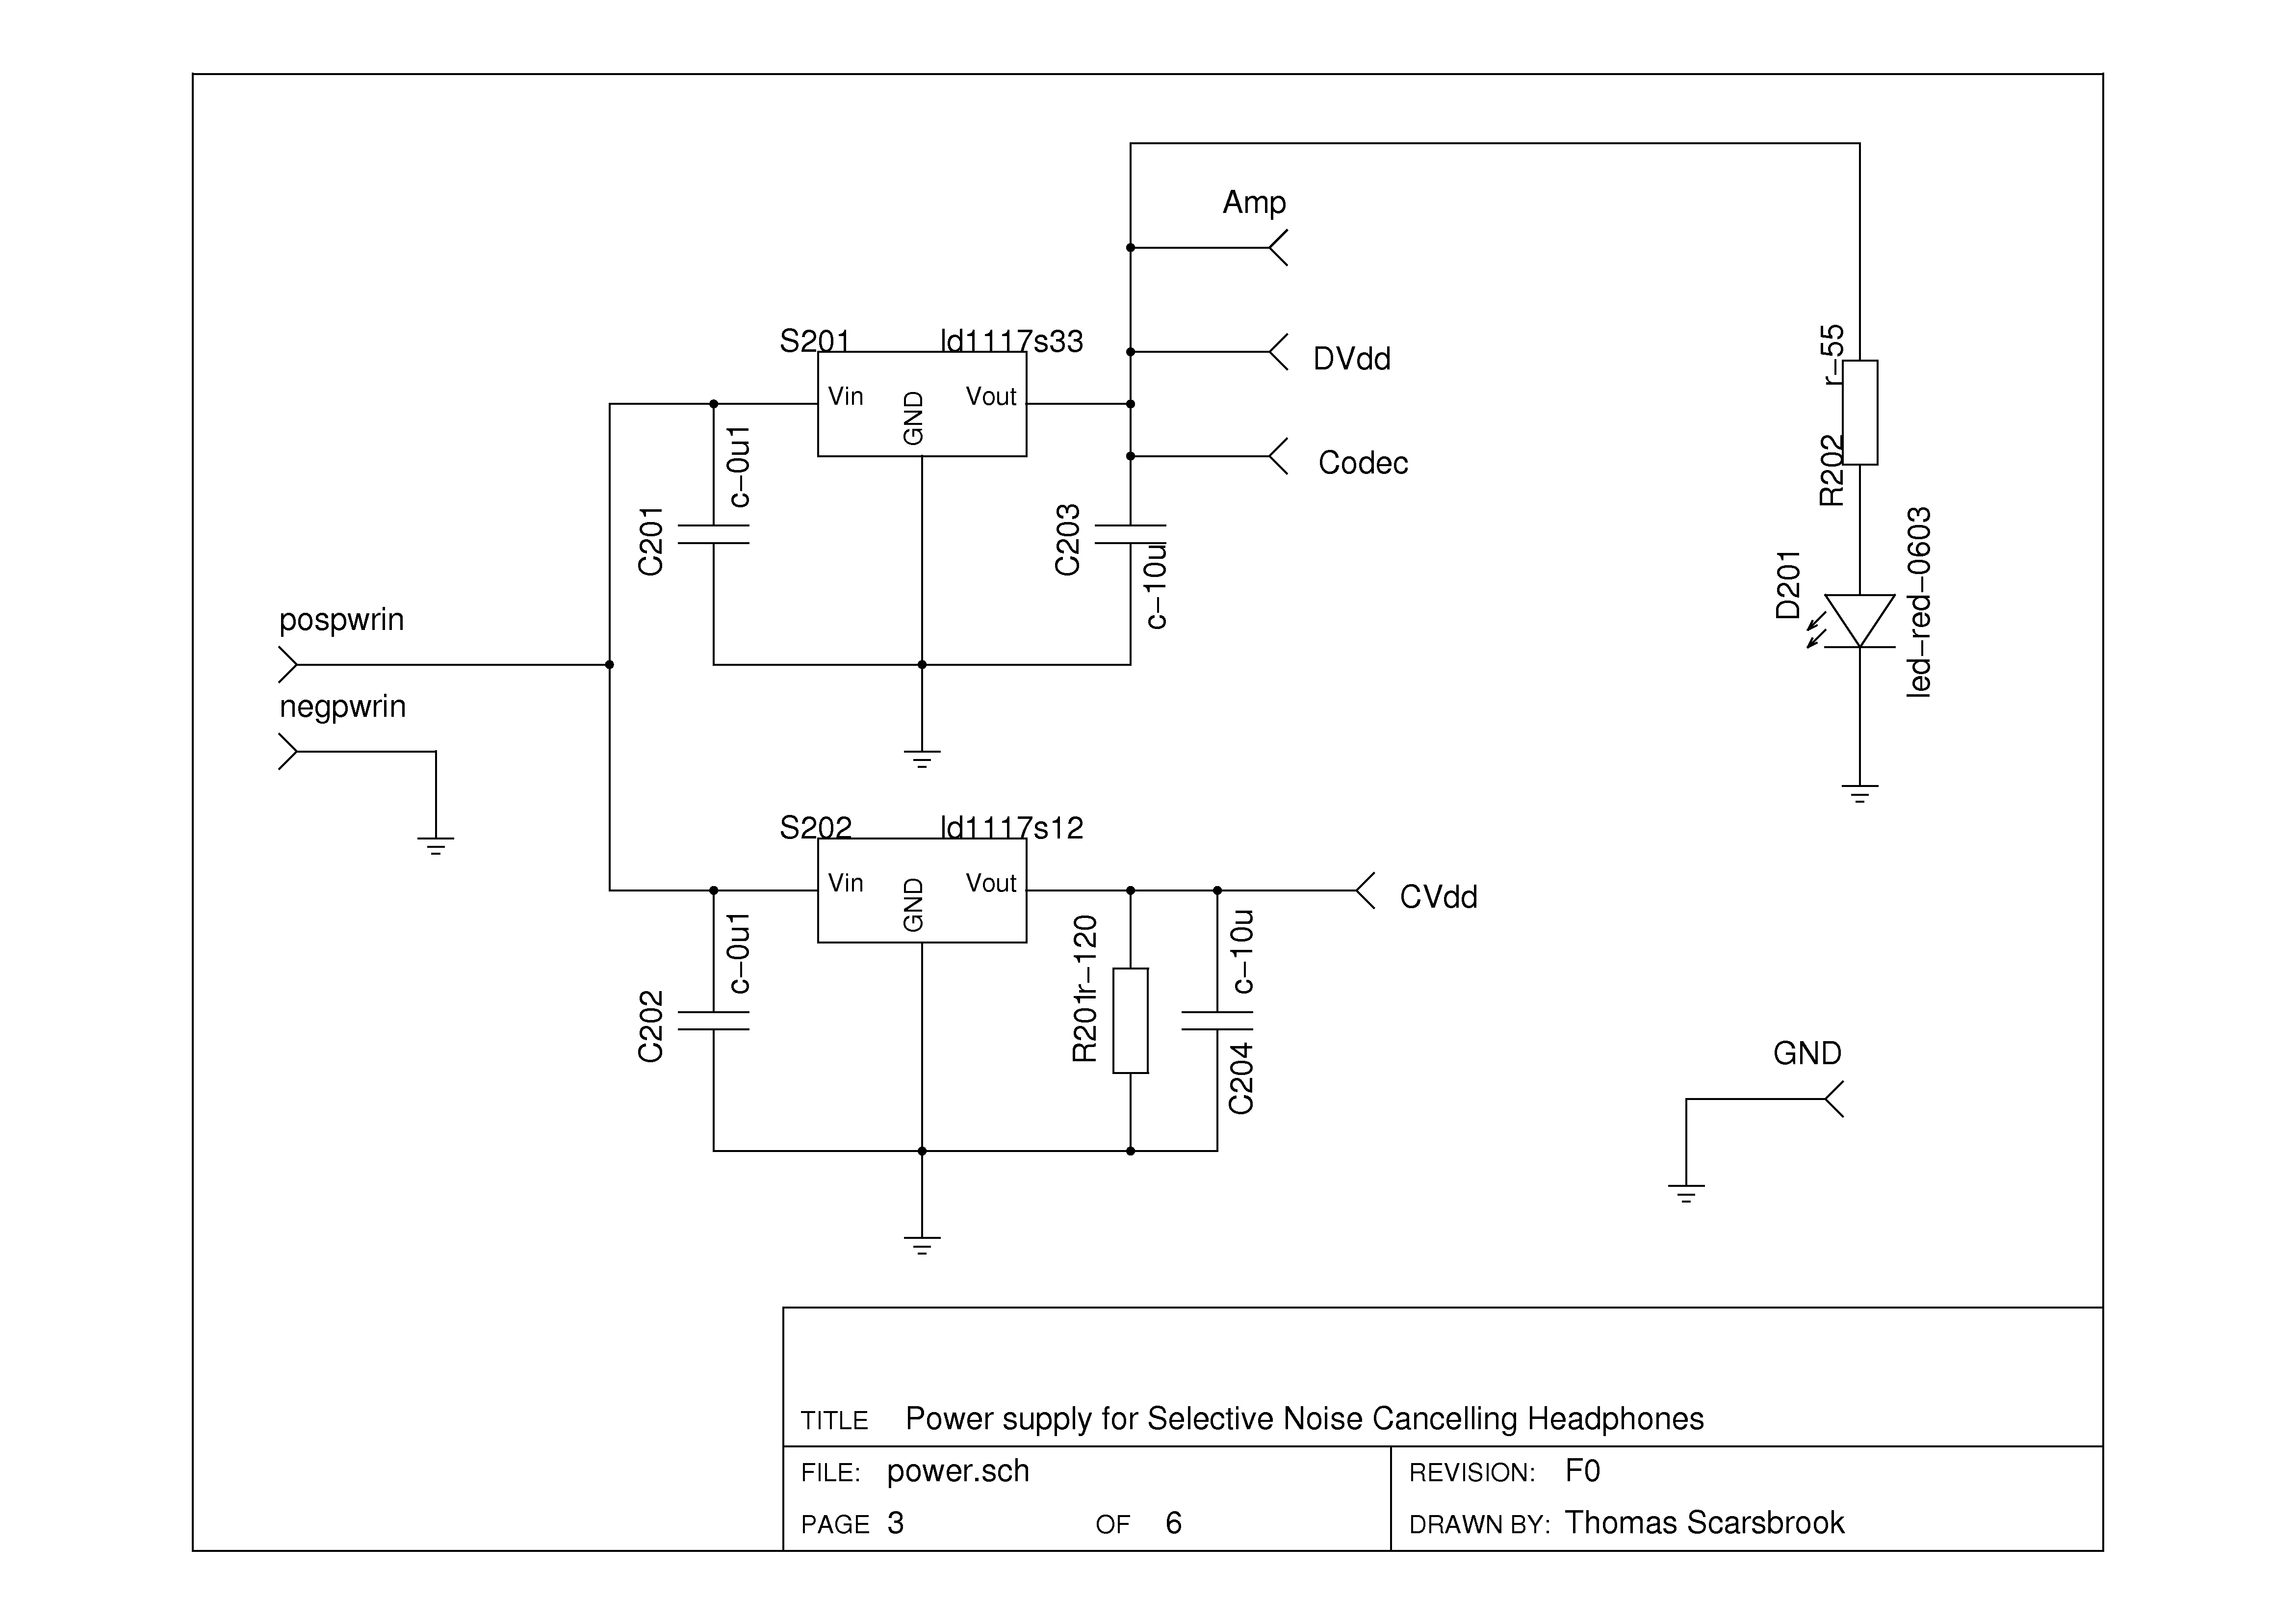
\includegraphics[width=\textwidth]{./img/power.png}
	\caption{The schematic of the power regulation for the projects PCB}
	\label{fig:powersch}
\end{figure}

\noindent In order to account for this two voltage regulators were obtained, one providing the 3.3V required by the DSP I/O and other circuitry, and the other providing the 1.2V required by the DSP core.
Both of these regulators were capable of providing 1.2A, which is in excess of the current requirements of the devices.
An LED was connected to the 3.3V rail to show when power was being provided, regardless of state of the rest of the system.

\begin{table}[H]
	\centering
	\begin{tabular}[c]{| l | c |}
		\hline
		\multicolumn{2}{|l|}{3.3V rail}\\
		\hline
		Component	& Draw (mA)	\\
		\hline
		DSP I/O		& 75	\\
		Codec		& 35.1	\\
		Clock Generator	& 160.6	\\
		Amplifiers	& 2	\\
		\hline
		Total		& 272.7	\\
		\hline
		\hline
		\multicolumn{2}{|l|}{1.2V rail}\\
		\hline
		Component	& Draw (mA)	\\
		\hline
		DSP core	& 625	\\
		\hline
		Total		& 625	\\
		\hline
	\end{tabular}	
	\caption{The current requirements of the various components in the circuits}
	\label{tab:pcbcurrentdraw}
\end{table}

\subsection{PCB}
Various things had to be taken into consideration for the PCB design.
The PCB was designed in gEDA PCB, as I had used the software previously.

\subsubsection{Coupling}
For starters the high frequency switching involved in the digital portion of the system could introduce a lot of noise which could distort the signal from the analogue portion.
This would largely be seen as current being drawn along the ground plane, introducing a rapidly changing voltage gradient across it.
While this isn't as much of an issue for the digital portion, as there are margins around each voltage level, the analogue portion would suffer significantly, especially if the noise is introduced after the signal conditioning stage.
In order to mitigate this, the analogue circuitry has a separate ground plane to the digital.
Obviously these two ground planes still need to be connected to the same external connection, so they connect at this point, meaning minimal chance of currents flowing through the other portion of the system.
These separate planes can be seen in figures \ref{fig:pcbtop} and \ref{fig:pcbbottom}.
The digital ground planes are the red and light green planes respectively, whilst the analogue grounds are grey and dark green.
\\
\\
In order to place the analogue circuitry on its own ground plane, it had to be segregated from the rest of the circuitry.
This style was maintained with the rest of the layout, where circuits with different functions were kept separated from the rest.
Power kept separate from the DSP, kept separate from the codec, etc.
An additional benefit arose from this, where signals travelling between parts of the system were travelling a short distance reducing the effect of noise.
An example of this is the clock generator feeding the codec.
The 12MHz signal it provides would generate a large amount of noise, however as it is kept in a segment with the codec IC itself the signal has a very short distance to travel.
As such this signal did not interfere with other signals as there was no need for it to pass near them.
Also there was a portion of ground plane between it and other signals, preventing it from passing over.
\\
\\
Another way to help mitigate the noise effects is to place decoupling capacitors across the power rails near each IC.
This is something that is required with the digital systems as well as the analogue circuitry, as they are still susceptible to this noise effect albeit less so than the analogue.
Some of these decoupling capacitors can be seen around the codec and clock generator, however the more obvious ones are those around the DSP.
Due to its size and complexity the DSP requires more decoupling than the rest of the circuitry.
Multiple sizes of capacitors were used around the DSP.
In opposing corners of the DSP a 10$\mu$F capacitor was placed to remove lower frequency components and to give a reasonable power storage against drops.
Then around the edge of the DSP, right next to the pins that required them, smaller 1$\mu$F capacitors were placed to remove high frequency components right at the power entry.


\subsubsection{Layers and Packaging}
There are various different packages available for the components to be used on the PCB, and which packages are used affect the construction of the PCB.
The first, basic decision to be made was whether to use surface mount components, or through hole components.
Due to the low power nature of this system this choice was remarkable simple.
Using through hole components would require more physical space above and below the PCB surface than surface mount components, and would be more bulky width ways.
Also the location of the pin holes would have taken more space than the surface mount pads, as they require space on both sides of the PCB.
Finally some components are limited in what packages they are available in.
For example the DSP was only available in surface mount packages.
As such there was no benefit to using through hole components, therefore surface mount ones were chosen.
\\
\\
The DSP was only available in two varieties of packaging, Quad Flat Package (QFP) or Ball Grid Array (BGA).
These packagings had an effect on not only the footprint required, but also pin availability and the speed the DSP could run at.
BGA had 272 pads arranged in a ring, 4 pads wide, around the underneath edge of the IC.
In order to connect to all these pads multiple levels were required, most likely requiring power and ground to be carried on separate layers on the PCB.
Increasing the PCB to 4 layers to allow for this would drastically increase the cost of the PCB, ~\pounds180 rather than the ~\pounds80 paid.
Routing the connections in between the pads and locating the decoupling capacitors would have been rather difficult.
Also there is then an issue in terms of production.
A BGA package requires soldering onto the board in an oven.
On the plus side, in this package the DSP was available in speeds up to 300MHz.
\\
\\
On the other hand QFP has all the pins located across the four sides of the IC, and therefore only provides 208 pins due to the reduced area to connect with.
However all the pins of the package could be physically accessed externally, meaning that routing around them becomes much easier, also only a single layer is required to mount the device.
Soldering the package to the board becomes an easier task too, and a standard soldering iron can be used.
QFP loses out on the speed side though, the only speed available in a QFP package is 200MHz.
\\
\\
Taking these into account it was decided to use the QFP package in this project.
While fewer pins are available to the user, none of the pins that became unavailable were required by this project, as such the loss of them was not an issue.
The slower speed was a greater factor, however it was outweighed by the cost of manufacture that the BGA would have required, and testability.
Due to the fact that all the pins of the QFP package were physically accessible by the user, testing would be easier as they can be probed, whereas the BGA package does not allow this.
\\
\\
In order to reduce the size of the board required, and to ease routing, and aid the placement of decoupling capacitors near the power connections, a two layer PCB was used.
This second layer allowed the decoupling capacitors to be placed directly beneath the pins they would connect to, reducing the distance from the pins and therefore reducing the amount of noise that could appear on the line.
However the more significant advantage was the ability for tracks that would otherwise conflict pass over each other.

\subsubsection{Debugging Headers}
Due to the fact this system was under development, the PCB would require vigorous testing after production.
In order to aid this testing a load of headers were placed between sections of the system, thus allowing the sections to be tested in isolation.
Not only could the output of a system be measured without the following stage affecting it, but also the input could be assigned manually without the preceding stage interfering.
Key placements of these headers were between the power and any other portion of the system, between the audio connections and the rest of the system, and on the interface between the analogue and digital portions of the system.


\begin{figure}[H]
	\centering
	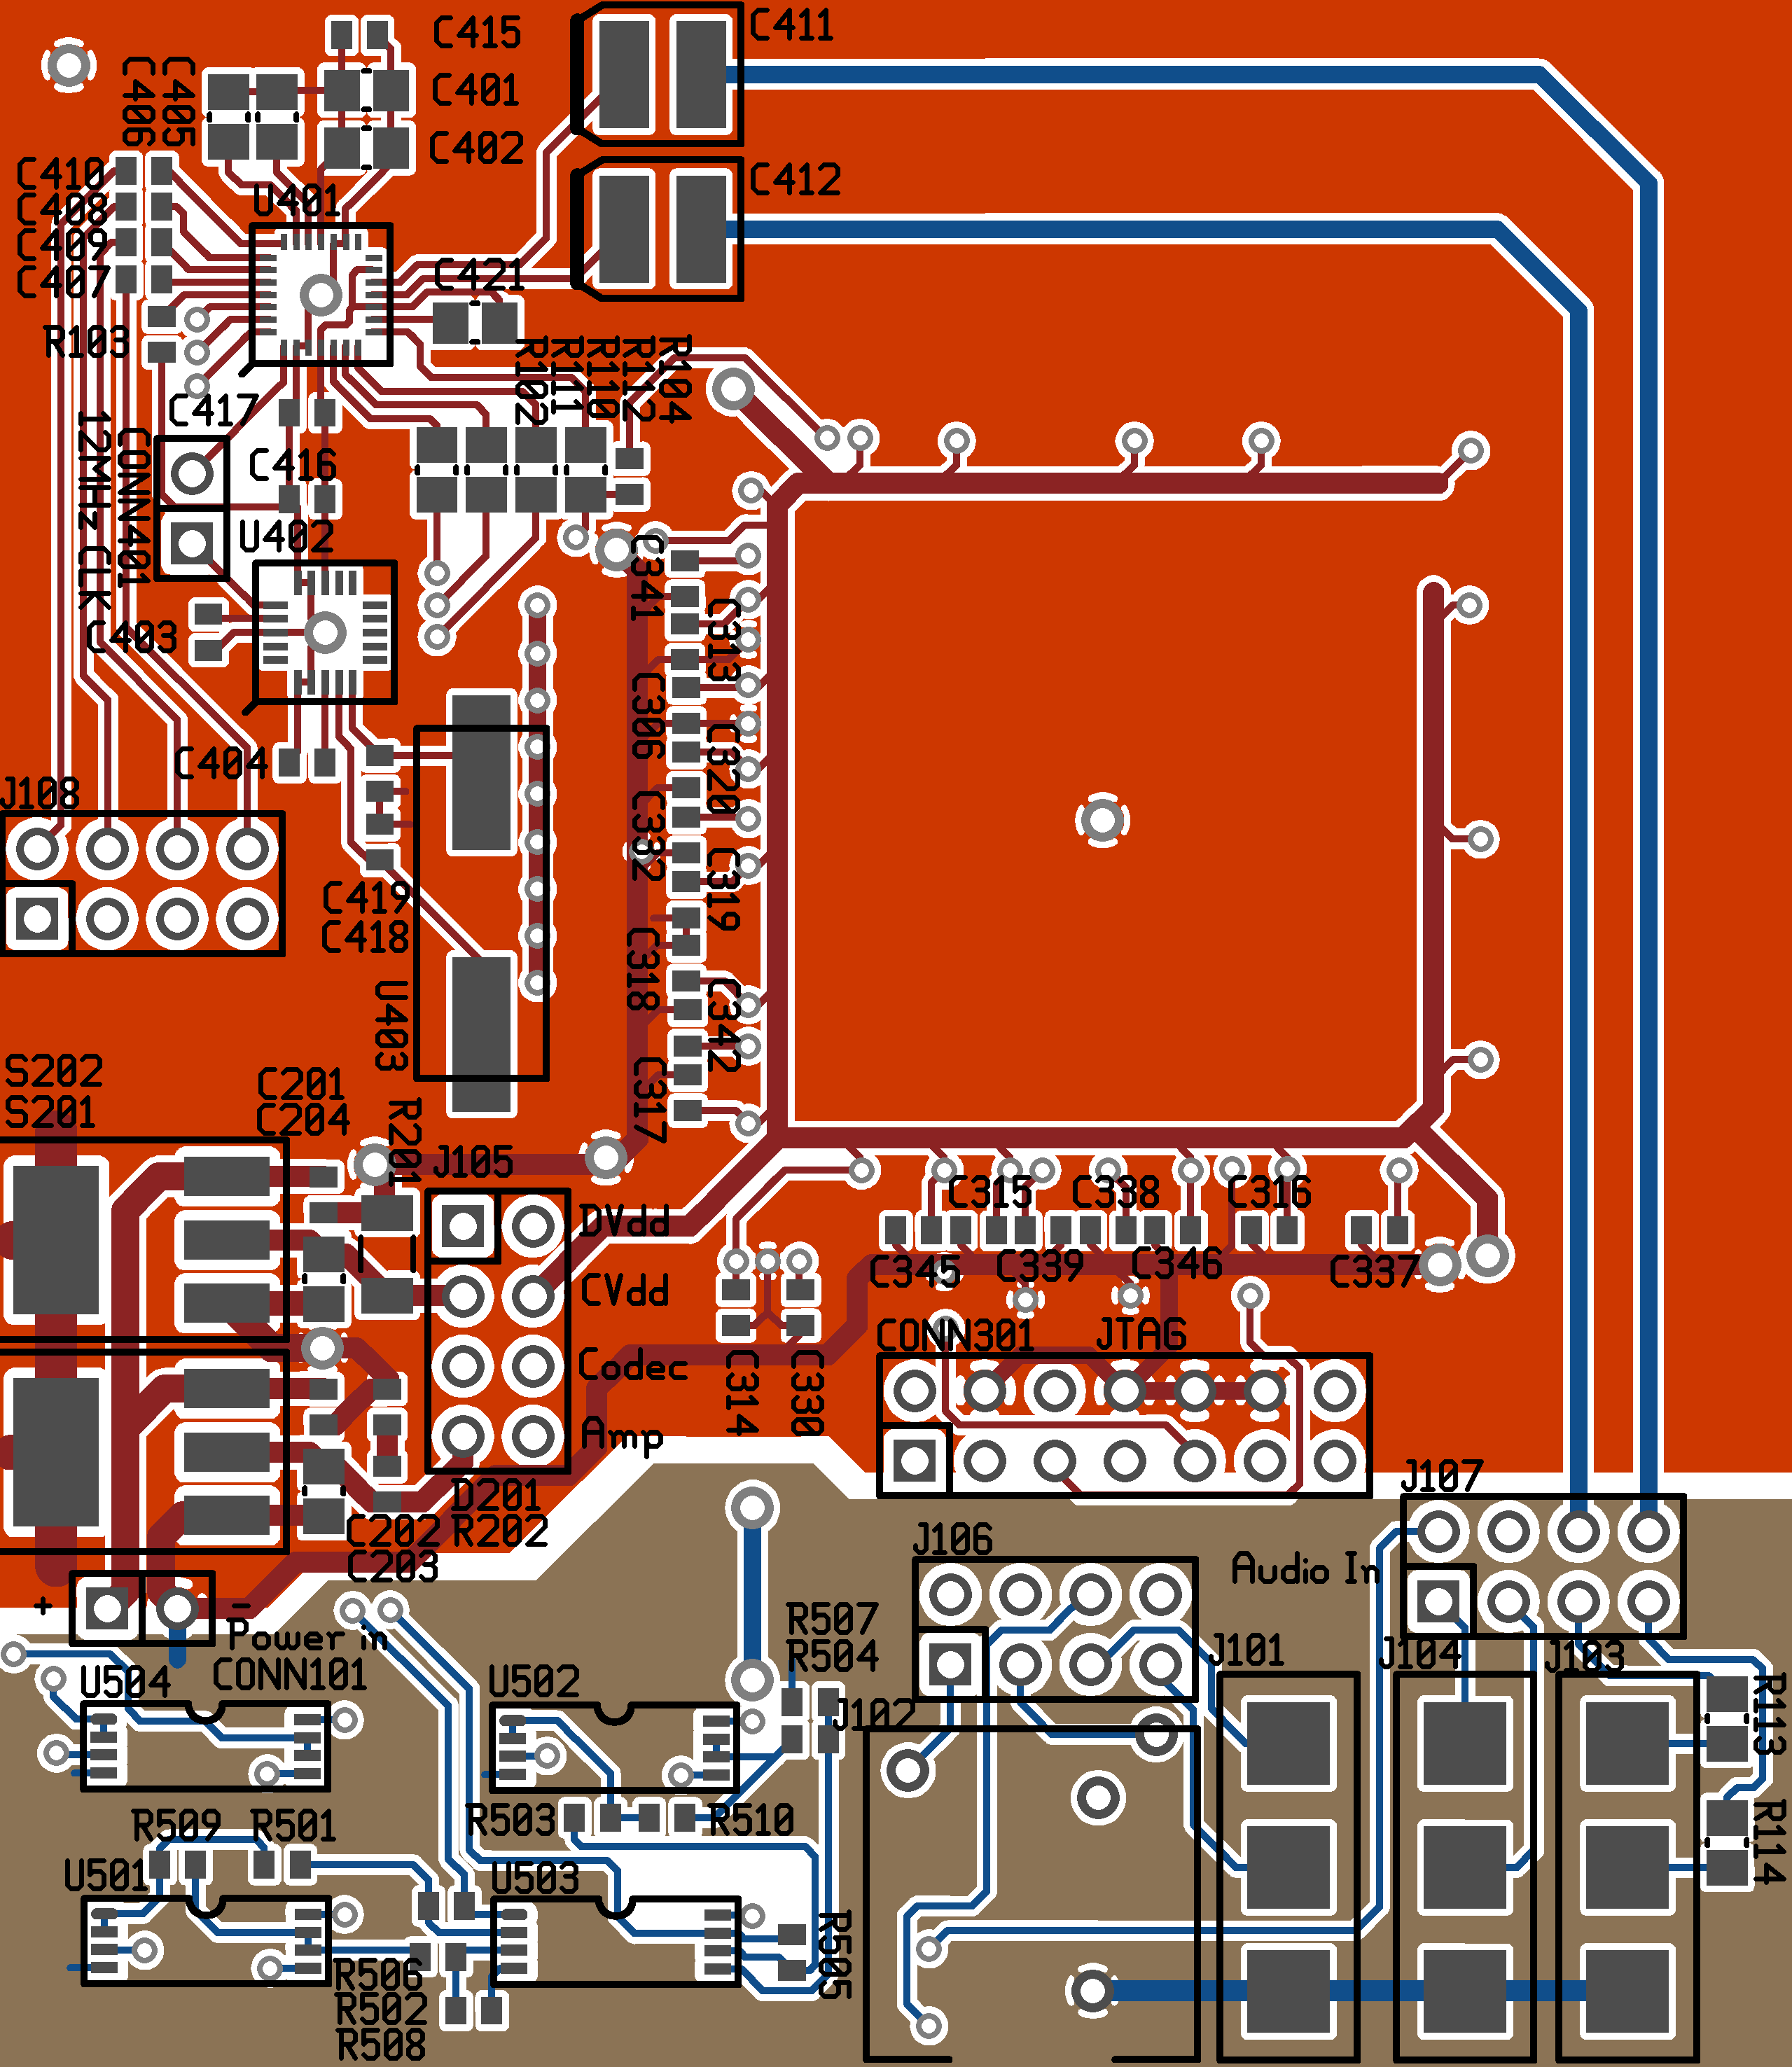
\includegraphics[width=280px]{./img/overview_top.png}
	\caption{The top side of the PCB}
	\label{fig:pcbtop}
\end{figure}
\begin{figure}[H]
	\centering
	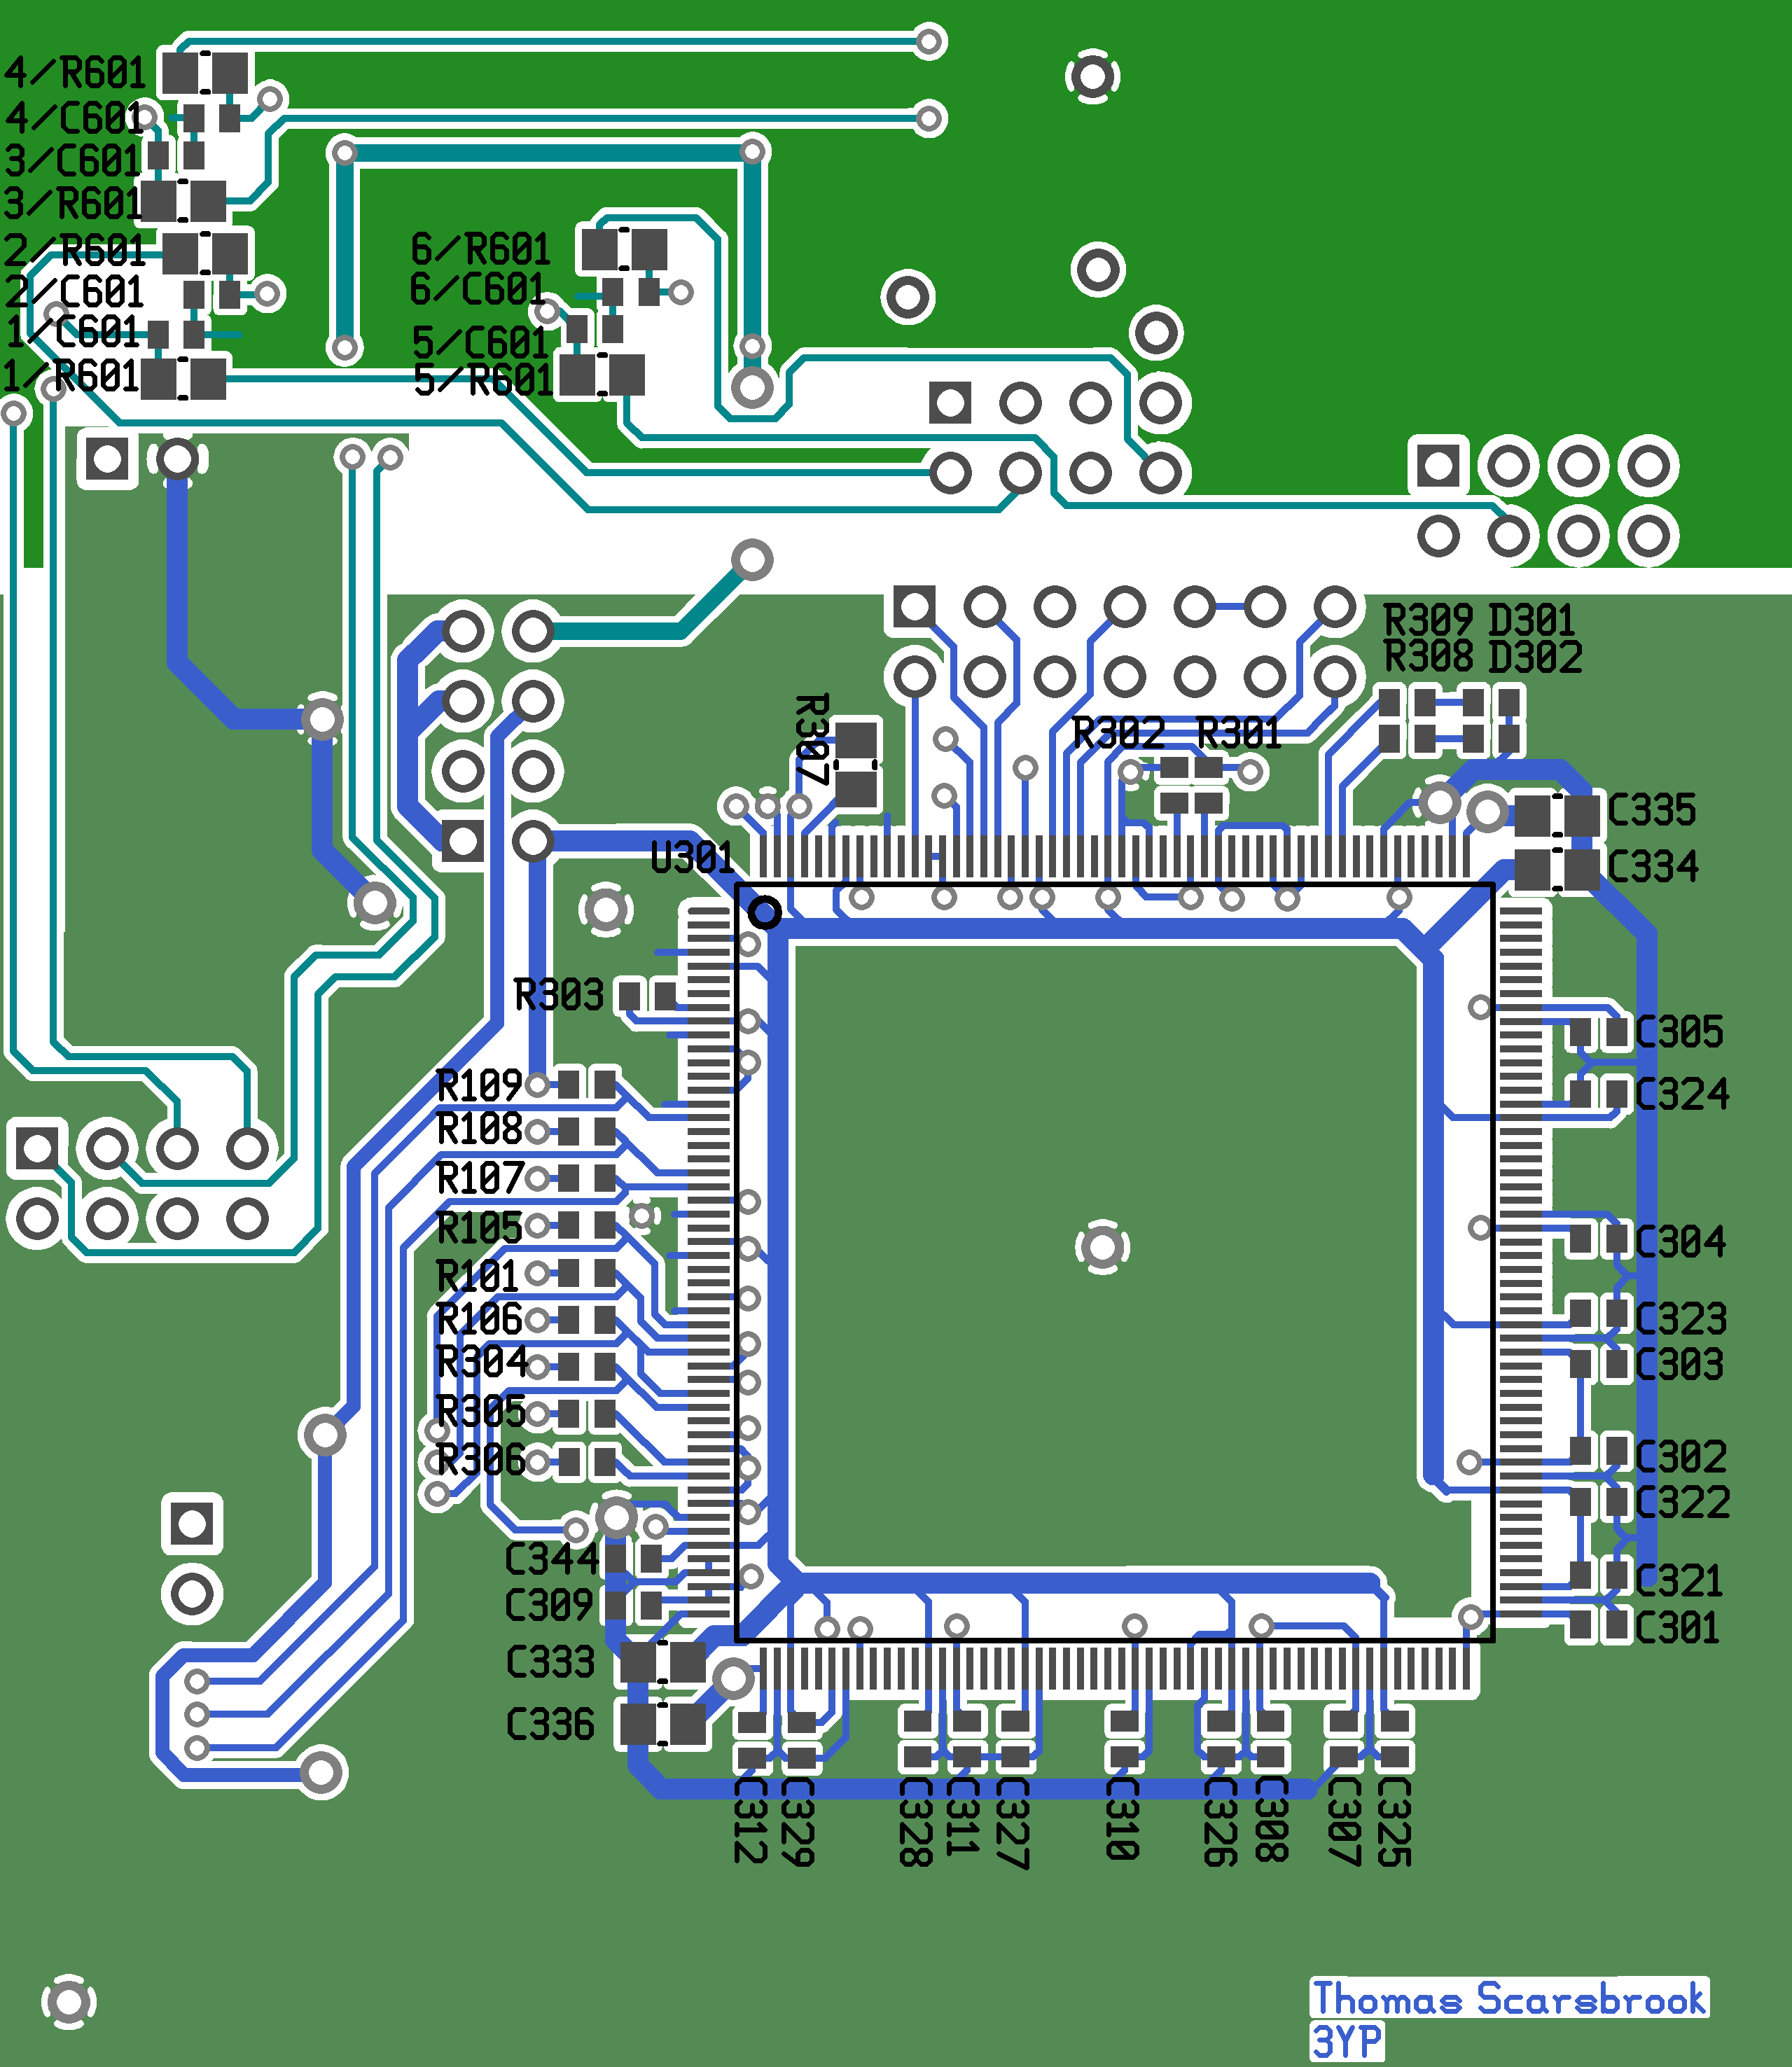
\includegraphics[width=280px]{./img/overview_bottom.png}
	\caption{The bottom side of the PCB}
	\label{fig:pcbbottom}
\end{figure}


\section{Software}
Many decisions were made in the implementation of the algorithms in this project.
Some of these decisions affected just the correlation method, some just the LMS method, and some that affected the project regardless of methodology.
Here these decisions are discussed, starting with the decisions that were method independent, then covering each of the method specific ones in turn.

\subsubsection{Language}

The algorithmic side of the system was implemented in the C programming language, due to the amount of control it provided and the fact that the available compilers required C.
This gave a large degree of control to the various peripherals built into the DSP, specifically a nice interface to the McBSP registers for communication with the codec, and the GPIO port for using the debugging LEDs.
The disadvantage this introduced was that built in data types and the available functions that could be acted upon them were a bit more restrictive than those used in the modelling with matlab.
As such the desired structs and functionality for the ring buffers (discussed below) had to be designed and developed manually.
This also affected the algorithms themselves, as each value had to be dealt with individually, whereas matlab could perform matrix based operations.

\subsubsection{Ring Buffers}

Some data needed to be stored in the DSP for the algorithm to work, whether the correlation method or the LMS method.
There are a few ways to achieve this.
One option is an array.
This would give the advantage of a simple system, whereby the latest value is loaded into the array.
The issue then arises on how to determine the location in the array to load the value, and how to maintain a consistent amount of storage.
If there's no wrapping around at the end of the array, then one of two options are available.
Either the new value is entered at the beginning of the array, and all other values get shifted along.
This method is very heavy on resources as it requires all the values in the arrays to be moved for each new sample.
The alternative is that the amount of data available for each sample varies, dropping down to just a single sample at times during the analysis.
This latter method is basically unacceptable for this project, it would result in the algorithm being unable to respond at portions of the time.
Alternatively the option of wrapping round at the end of the array, this is the first step towards a ring buffer.
Wrapping around at the end of an array removes the need to shift all values along upon receiving a new sample, it also prevents varying available data sizes.
However it then introduces an issue of keeping track of the location in the array and how to deal with the wrap-around.
Multiple variables would have to be stored and whenever a piece of code works with the array it would have to keep track of the wrapping around, introducing a large margin for error in coding.
\\
\\
To eliminate this, a ring buffer struct was developed.
This allowed the required variables to be linked directly with the array being dealt with, and shifting through the array could now be done with a standard function that only required a single argument.
The result of using ring buffers was that the code became simpler to write and deal with, reducing room for error, however this came at a cost.
Using a simple array based method would have resulted in minimal computational effort in shifting through the array, with ring buffers more effort was required, slowing down the overall operation.
Thanks to the speed of the DSP the number of clock cycles this would cost was minimal, and as such ring buffers were used for the remainder of the project.
\\
\\
The use of ring buffers provided other advantages.
After implementing the different algorithms optimisation was required, and the ring buffers assisted with that greatly.
For example, when calculating the mean of the data in the buffer, it is known that the next sample in the buffer, regardless of position in the buffer, is the oldest sample.
Therefore, in order to determine the mean and additional variable could be stored holding the sum of the values in the buffer, and on a new sample the oldest sample can be subtracted, the new value added, and then a single division made.
As a result calculating the mean is reduced to a single addition, single subtraction, single division, and a single shift through the buffer, rather than an addition and shift for each value in the buffer, followed by a division.
This is a huge time saving, and as the number of clock cycles is heavily restricted a saving this large is a real advantage.

\subsubsection{Code Isolation}
In order to ease the writing and testing of the code, separate parts of the code were written in separate files, with minimal requirements from other files.
All the code that interfaced with external devices, such as the code relating to the codec communications, was especially separated out, with only functions
to get and send data used externally.
This gave the advantage that all the algorithmic code was cross platform, enabling it to be tested on normal computer systems.
Of course to test it on a normal computer system, the I/O calls and the codec interface were no longer valid, so had to be mimicked.
This mimicking was achieved through a minimalistic block of code which simply read from a file and wrote to the console.
\\
\\
This ability to test it cross platform proved especially useful when a ring buffer pointer was not being shifted through the buffer correctly, resulting in a memory leakage.
The DSP just followed its programming and continued, overflowing and overwriting program memory.
This resulted in unexpected crashes on both the DSP and its debugger, which just looked like the code had frozen.
When tested in a linux terminal, the memory overflow was detected and indicated as a segmentation fault with a complete stack trace, allowing the bug to be very easily traced.

\subsubsection{Self Written}
In this project none of the C code used was taken from an available library or provided by anyone not involved in this project.
Some of the matlab code written during the modelling used inbuilt functions to begin with, in order to produce proof of concept, however then was re-written to remove these external functions.
\\
\\
There were multiple advantages to writing all the code.
One of these was the advantage of using the desirable data structures, in particular the ring buffers.
While many libraries available deal with ranges of data, they generally expect arrays and do not provide the capability to deal with the ring buffers used in the rest of the project.
This would result in having to resort to the alternatives, resulting in serious losses to functionality.
\\
\\
Of course, no advantages come for free, and as such there were multiple disadvantages to this approach.
The most obvious one being that all the code had to be written and tested, whereas this would have been done extensively with any available libraries.
On top of this, libraries are available for the DSP which achieve a variety of functions, and have had the assembly code hand optimised by the manufacturer, Texas Instruments (TI).
These optimisations were lost, resulting in slightly slower code.
However many of these libraries were incompatible with the data structures used by the rest of the system, so the losses in optimisations here were made up for through optimisation in other ways, as previously discussed.

\subsection{Correlation}

After writing the code for the correlation algorithm, a problem was discovered.
The algorithm for cross-correlation requires the use of the mean in the calculation.
Whilst the mean could be calculated easily due to the advantages provided through the use of ring buffers, there was additional issues with the inserting this mean at the correct point in the calculation.
The entire buffer had to be iterated through after the calculation of the mean, and a calculation performed at each step.
This second calculation was more intensive than the calculation of the mean would have been.
This produced a severe draw on the processing power of the DSP, and resulted in the system taking approximately 7 seconds between each sample.
As the codec operated at 48KHz, this meant that the code was operating about three hundred thousand times too slow.
\\
\\
Two options presented themselves in order to reduce this issue.
Firstly the length of the buffers could be reduced.
This would have been a simple fix, and would have drastically speeded up the algorithm.
On the flip side of the coin however, reducing the buffer size by enough to produce a suitably fast algorithm would have removed so much information than would have been desirable for accurate cancelling.
Another effect of shortening the buffers would be that the headphones could no longer deal with as long a difference between the heard signal and the noise signal.
As a result, the cancelling effect would be reduced.
\\
\\
The other option would be to optimise the code by as many means possible, by looking for loopholes in how the algorithm iterates through the loops.
\\
\\
To a certain degree both methods were used to speed up the system, however were not effective enough.

\subsection{LMS}
\label{ssec:implelms}
The LMS code acted in three stages; calculate output, generate feedback, update weights.
The first of these stages, calculating the output, involved iterating over a loop summing up the various taps.
The weights were stored in an array, and matched against the values in the ring buffer by producing a new pointer for it, and shifting it round backwards.
After multiplying respective weights and stored values, the output of this filter is then played out through the headphones.
\\
\\
The seconds stage involved the generation of a virtual feedback value to be used for the final stage.
The generation of this assumed that the sounds reaching the external microphone of the headphones were the same as those reaching the eardrum.
This assumption was slightly dangerous as it did not account for the demanded sound signal, which would be reaching the eardrum also.
\\
\\
The final stage involved updating the array of weights to optimise the cancellation, based on the feedback.
The algorithm for calculating the updated weights works on the basis of minimising the power of the virtual feedback signal.
At this point the assumption made in the second stage is validated.
As different signals are superimposed together the overall power of the summed signal changes, therefore summing the demanded signal onto the heard signal would cause the power to shift.
If the demanded signal happened to be that of the noise signal then the power of the summed signal would be increased.
Because this summed signal correlates well with the noise signal, the LMS filter will update to double the value they'd otherwise be at in order to reduce to the minimum power level.
This will cancel not only the noise that reaches the ear, but also the demanded signal, the result of which will be that the user will temporarily be unable to hear the demanded signal.
A similar effect could be observed if the demanded signal happened to be the inverse of the noise signal, the difference being that the filter weights will be updated to zero.
The user will experience the same 'deaf' effect.
By keeping the demanded signal out of this virtual feedback loop it is guaranteed that the demanded signal will not be cancelled out, as only components in the heard signal will be acted upon.
Once the updated weights have been calculated and stored in the array the loop repeats.
\\
\\
As I write this I discover a serious design flaw in the summation of the heard and demanded signals before sampling.
The justification for virtual feedback is nullified by the fact that the demanded signal is added to the heard signal before sampling.
The solution would be to put the instrumentation amplifier in the output feed.


\chapter{Testing}

\chapter{Evaluation}

\chapter{Conclusions}

\bibliographystyle{plain}
\bibliography{sources}

\appendix
\chapter{Weekly Tracker Samples}
\label{appendix:weeklytracker}

\chapter{PCB Costings}
The costings of the components for the PCB.
The total cost came to \pounds196.90

\begin{table}[H]
	\centering
	\begin{tabular}[c]{| l | l | l | p{50px} | l | l | l |}
		\hline
		\multicolumn{7}{|l|}{MicroControllers} \\
		\hline
		Item	& Component Name& Supplier & Part	& No.	& Unit  & Line \\
		\hline
		DSP	& tms320c6713bpyp200	& Farnell	& 1214441	& 1	& \pounds24.51	& \pounds29.42	\\
		Codec	& wm8988		& Farnell	& 1776294	& 2	& \pounds2.84	& \pounds6.82	\\
		Clock Gen.	& bu2796	& Farnell	& 1716138	& 2	& \pounds0.83	& \pounds1.99	\\
		Dual Op-Amp	& ap358sg	& Farnell	& 1825347	& 10	& \pounds0.08	& \pounds0.96	\\
		\hline
		\multicolumn{7}{|l|}{}\\
		\hline
		\multicolumn{7}{|l|}{Resistors} \\
		\hline
		Item	& Component Name& Supplier & Part	& No.	& Unit  & Line \\
		\hline
		10K\textohm	& r-10k	& Farnell	& 1469748	& 50	& \pounds0.013	& \pounds0.78	\\
		8K2\textohm	& r-8k2	& Farnell	& 9334904	& 50	& \pounds0.01	& \pounds0.60	\\
		1K\textohm	& r-1k	& Farnell	& 9332383	& 50	& \pounds0.025	& \pounds1.50	\\
		120\textohm	& r-120	& Farnell	& 9337059	& 50	& \pounds0.011	& \pounds0.66	\\
		55\textohm	& r-55	& Farnell	& 1500641	& 50	& \pounds0.015	& \pounds0.90	\\
		33\textohm	& r-33	& Farnell	& 1500704	& 50	& \pounds0.016	& \pounds0.96	\\
		8\textohm	& r-8	& Farnell	& 1577385	& 50	& \pounds0.047	& \pounds2.82	\\
		\hline
		\multicolumn{7}{|l|}{}\\
		\hline
		\multicolumn{7}{|l|}{Capacitors} \\
		\hline
		Item	& Component Name& Supplier & Part	& No.	& Unit  & Line  \\
		\hline
		220uF	& c-220u& Farnell	& 1865004	& 5	& \pounds1.10	& \pounds6.60	\\
		10uF	& c-10u	& Farnell	& 1658212	& 10	& \pounds0.115	& \pounds1.38	\\
		4u7F	& c-4u7	& Farnell	& 1759427	& 100	& \pounds0.018	& \pounds2.16	\\
		1uF	& c-1u	& Farnell	& 1759398	& 100	& \pounds0.006	& \pounds0.72	\\
		100nF	& c-0u1	& Farnell	& 1759123	& 100	& \pounds0.005	& \pounds0.60	\\
		1nF	& c-1n	& Farnell	& 1759088	& 100	& \pounds0.005	& \pounds0.60	\\
		8pF	& c-8p	& Farnell	& 1759051	& 100	& \pounds0.006	& \pounds0.72	\\
		\hline
		\multicolumn{7}{|l|}{}\\
		\hline
		\multicolumn{7}{|l|}{Connectors} \\
		\hline
		Item	& Component Name& Supplier & Part	& No.	& Unit  & Line \\
		\hline
		2 pin	& cn-header2	& Farnell	& 1248140	& 10	& \pounds0.106	& \pounds1.24	\\
		8 pin	& cn-header2x4	& Farnell	& 1759051	& 8	& \pounds0.98	& \pounds9.41	\\
		14 pin	& cn-header2x7-box	& Farnell	& 8395926	& 2	& \pounds0.72	& \pounds1.73	\\
		Jack	& cn-st-jack	& Farnell	& 1217016	& 2	& \pounds1.36	& \pounds3.26	\\
		\hline
		\multicolumn{7}{|l|}{}\\
		\hline
		\multicolumn{7}{|l|}{Miscellaneous} \\
		\hline
		Item	& Component Name& Supplier & Part	& No.	& Unit  & Line \\
		\hline
		3.3V Regulator	& ld1117s33	& Farnell	& 1467779	& 2	& \pounds0.71	& \pounds1.71	\\
		1.2V Regulator	& ld1117s12	& Farnell	& 1467778	& 2	& \pounds1.02	& \pounds2.45	\\
		12MHz Crystal	& xtal-12m	& Farnell	& 1652551	& 2	& \pounds0.32	& \pounds0.77	\\
		Red LED		& led-red-0603	& Farnell	& 1465988	& 10	& \pounds0.23	& \pounds2.76	\\
		PCB		&	 	& PCB-Train	& 		& 2	& \pounds78.16	& \pounds78.16	\\
		JTAG Cable	&		& FTDI		& C232HM-DDHSL-0& 1	& \pounds18.50	& \pounds22.20	\\
		Headphones	&		& Play.com	& 3432806	& 1	& \pounds12.99	& \pounds12.99	\\
		\hline
	\end{tabular}
	\caption{Costs involved in the PCB production. Prices correct at time of purchase, line cost includes VAT, unit cost may not}
	\label{tab:pcbcostings}
\end{table}

\chapter{ICA}
Independent Component Analysis (ICA) is a method for separating different signals from a mix.

\section{Methodology}

\section{Limitations}
ICA has some limitations which must be met.
Some of these limitations would result in this algorithm being unsuitable for this project, though these limitations could potentially be circumvented through knowing the circumstances of use.

Under normal circumstances ICA requires at least as many sensors as signal sources.
Without this there isn't enough statistical variation for the different signals to be separated out.
This project only allows for two inputs, one in each ear, which would result in the use of ICA only working for 2 sound sources in the room, which is unlikely to occur, making the use of ICA pointless.
In order to solve this problem certain information about the location and construction of the headphones can be utilised.
The headphones are positioned inside the ear with the microphones pointing outwards.
The ear is shaped in order to direct sound inside the ear, also the microphones are rather directional resulting in 

\section{Implementation}
In the final project ICA was not implemented.
This was largely due to the unexpected length of time taken in implementing the noise cancellation algorithm.


\end{document}
